\documentclass[
  final,
  babelLanguage=british,
  %desktopVersion,
  printOnDemand,
  %showtrims,
  %overleaf,
]{anecdote}

\graphicspath{{./assets/photos/300dpi/}}
%\graphicspath{{./assets/photos/92dpi/}}

% Blurb page size: 5 x 8 inch (127 x 203.2 mm)
% Body text: 10.5 / 16 pt

\usepackage{local}

%% Details of the book
%% ===================

\title{Wordless Questioning}
\subtitle{an introduction to Buddhist meditation and reflection}
\author{Gambhīro Bhikkhu}
\publisher{Publicações Sumedhārāma}
\date{2022-05-05}
\editionInfo{\textit{First edition}, 2022}
\ISBN{978-989-8994-35-6}

% === Metadata ===

\hypersetup{
  pdftitle={\thetitle},
  pdfauthor={\theauthor},
  pdfcopyright={Copyright (C) 2022, \theauthor},
  pdfsubject={an introduction to Buddhist meditation and reflection},
  pdfkeywords={Bhikkhu Gambhiro, meditation, Dhamma, Buddhism, RELIGION / Buddhism / Theravada},
  pdflicenseurl={https://creativecommons.org/licenses/by-nc-nd/4.0/},
  pdfcontacturl={},
  pdflang={en},
}

%% === Load further packages ===

%% === Hyphenation exceptions and corrections ===

\hyphenation{London}

\begin{document}

\frontmatter

\ifdesktopversion
\desktopCover{\includegraphics[height=\paperheight]{./desktop-cover-en.jpg}}
\fi

\cleartorecto
\thispagestyle{empty}
\vspace*{5em}

{\centering

{\Large\alegreyaSansScLightFont\selectfont\MakeLowercase{\textls*{\thetitle}}}\\[5pt]
{\chapterTitleFont\selectfont\itshape \thesubtitle}

\vfill

{\chapterTitleFont \theauthor}

\vspace*{2em}

}



\cleartoverso
\thispagestyle{empty}

{\copyrightsize
\centering
\setlength{\parindent}{0pt}%
\setlength{\parskip}{0.8\baselineskip}%

\thetitle\\
by \theauthor

Published by \thePublisher

ISBN \theISBN

Copyright \copyright\ \theauthor\ 2022

Editor: Kovilo Bhikkhu

Illustrations: Madalena Scafuro

This book is available for free download at

\href{https://forestsangha.org/}{www.forestsangha.org}

\href{https://a-buddha-ujja.hu/}{www.a-buddha-ujja.hu}

\vfill

This work is licensed under a Creative Commons\\
Attribution-NonCommercial-NoDerivatives 4.0 International~License.

Produced with the \LaTeX\ typesetting system, set in Crimson~Roman and Alegreya Sans.

\theEditionInfo

}


\cleartorecto
\aliaspagestyle{chapter}{empty}

\tableofcontents*

\clearpage
\aliaspagestyle{chapter}{bottomcenter}

\openany
\hypertarget{introduction}{%
\chapter{Introduction -- A Proper Purpose}\label{introduction}}

A sense of disturbing suffering, painful loss or sense of confusion
where nothing makes sense -- these feelings stop us in everything we
were doing, and start the circles of thinking about what to do and why
is it this way. A sense of meaninglessness and being locked into a
situation becomes a heavy burden with an overriding sense to free
ourselves from it. It is not clear how, but we start asking questions
and investigating the teachings. We don't know how to do it -- but the
aspiration to be well is there.

Human beings can overcome confusion and flourish in their lives.

The view and attitude we cultivate is that suffering doesn't come from
being alive, but from a distorted understanding of it. We crave and want
to hold onto experiences which are always going to change, and that
sounds like suffering, doesn't it? It sounds meaningless, limited and
locking us in.

Cultivating right view allows for space and freedom around the
limitations of life, and we don't need so much for living one day. When
you feel that you have what you need to live this day well, the
expression of living with that understanding is contentment, gratitude
for life and energy to continue the work of a human being.

We are flooded with good advice about `how to be happy', so what's the
problem? If all it took was good advice, we would be all enlightened
long ago. All the good things we should do, the kind of person we should
be -- one source says we should be tough and fearless, another says we
should have universal compassion. It is a special kind of suffering to
read it all.

Or should we have \emph{Nibbāna}? Is that the right thing? The meaning
of the word is \emph{going cool}, as a fire ceases to burn and goes
cool. A craving to have or attain it would be more fuel for the heat and
burning of becoming. But \emph{Nibbāna} is the coolness of ceasing to
burn, so we should become the non-becoming? The thinking goes,
`\emph{What?}' Here is the genius of the Buddha -- he is teaching that
thinking and becoming won't get us there. If we are creating it, adding
or removing it by thinking, it will be as limited as before. We are not
free by becoming the right thing, but by recognizing that we can give up
the compulsion to continue becoming.

When we are happy in our activities and life is full of meaning, we are
not looking for answers and solutions, because we don't see any need for
them. This peace is often disturbed though, and we start asking
questions.

The best questions come to us in the form of `How should I understand
this well?' Watch what happens when you ask this. Discard the opinions
which present themselves as answers, and keep returning to this open
attitude of knowing the present.

Both joy and sorrow are part of natural processes, but if we don't
understand them, we see one as a reward and the other as punishment,
life never seems to be fair and always out of our control.

Could it be something else the matter? At least we can imagine the
possibility that there is something we can learn. A turning point occurs
when we are not sure about our opinion and we stop to look at the
experience to investigate. Understanding how one thing leads to another
is liberating on a fundamental level, which applies either in times of
joy or sorrow. The experience of such an understanding is freedom in the
mind and contentment in the heart. Practising to live with this freedom
and contentment is a proper purpose of meditation.

Meditation, in general, may be simple relaxation. In the context of the
Buddha's teaching, and when we are going through suffering, meditation
refers to calming the mind and developing insight into the natural
processes of our experience.

It doesn't seem to ask too much, does it? Stopping the hurry for a bit
of clarity, building up some understanding by watching what is going on,
life might start to make sense and we can relax the tension a bit.

We start with assuming that we don't know. Consider how narrow our
attitude is when we start with `\emph{I've seen this, I know this}'.
Perhaps this is true. But I notice that when I try to use knowledge to
solve a problem, my attention revolves around memories, thoughts and
opinions. While I am caught up in the past, the present experience
escapes my attention.

The instruction of the Buddha is to establish a careful intention to
meditate, putting aside the matters of the world for the moment.
Watching experience directly in the body, feelings, mind, and natural
processes as they are.

Contemplating our experience through watching the senses, the
impermanence of experience changes our attitude and perspective of it.
This is about understanding a process, not about gaining knowledge --
there is still no fixed thought or opinion which will become \emph{our}
knowledge -- but our trust is now in the awareness which can be
conscious of, and stay with the changing present. Letting go of our
fixed positions becomes the way forward, seeing with new eyes.

The practice of this understanding feeds back into \emph{what} we do and
\emph{how} we do it. This time, we are not blocked by confusion and
resentment about where we are now, and instead accept our work to be the
best version of ourselves. Life may still not be fair and not entirely
under our control, but now we know a deliberate practice which makes the
difference between a mental breakdown and understanding the facts.

The obstacles of the mind and heart are there because there is something
we have not yet understood with conscious awareness. After the
difficulties clear up, there is space and time to stop for joy and
gratitude.

It feels hopeless sometimes, and the thinking mind seems to have no way
to stop. The fundamental principle is that watching the mind develops
the mind. A wakeful, conscious awareness stops the compulsive
tendencies, which have been unknowingly, unseeingly driving us to the
same painful situations.

The word `Buddha' means `one who knows, one who is awake'. The source of
contentment in activity is that we continue to trust and practice this
wakeful awareness. We don't know what is going to happen tomorrow, but
we can learn to trust our capacity to practise this wakeful awareness in
the present.

Over the years I received much needed help and support to practice from
my teachers and monastic friends. We may not believe in ourselves that
we can be happy, but our teachers believe in us and wish us well. May
all beings overcome confusion and flourish in their lives.

{%
  \raggedleft
  Gambhīro Bhikkhu
  \par%
}



% Page 1 is the first page of the first chapter.
\mainmatter

\openright

\hypertarget{breathing-1}{%
\chapter{Breathing}\label{breathing-1}}

We watch the sensations of the breathing in the body, this alert
attention collects the mind around a stable object. The physical
sensations in the body are easy to notice as we breathe in- and out.

Why are we exhausted with all the thinking? The mind is jumping from
thought to thought, but we don't know where we are going and so we never
arrive: restless desire is exhausting. Sense-restraint gathers energy
and directs it, instead of letting it flow in every direction. Directing
attention to a neutral, steady sensation slows down the thinking mind.

Sit in a balanced, upright posture. The bones in the body sit on top of
each other like a small tower of stones. When balanced carefully, its
weight at the centre, we don't have hold it by muscle power, gravity is
enough to keep the body upright.

Breathing in, the cold air touches the tip of the nose. Let the abdomen
muscles draw in the breath, instead of expanding the chest to gain
volume. The air moves through the lungs and the abdomen expands; this
way of breathing lowers the heart rate and reduces anxiety. Relaxing the
muscles, the air leaves through the nostrils. There is no need to
control it with precision, it is enough to suggest this rhythm. The body
knows how to breathe, we take a step back and observe, like watching
waves wash in onto the shore, and then recede.

We don't have to tell ourselves what to think and how to feel. If we
want clear thoughts, it is best to first be silent and listen. We sit
and rest for a little while. When we are silent, either clear thoughts
will come on their own, or the mind will be content to stay with the
silence.

Restraint and directed attention is necessary for clear, conscious
thought -- and it brings peaceful gladness with it. The mind is content
and happy, we don't need much internal discussion. Sitting and
breathing, listening to the silence is a blameless joy in itself.

The right attitude is a careful balance. We establish a clear intention
to stay with the meditation object and leave other matters until a later
time, while maintaining an open attitude. Pushing and forcing ourselves
is not sensitive enough to what is happening. Operating from will-power
becomes rigid and obstructive.

A clear mind and good aspiration feels settled and cool, open for
changes. A forceful struggle feels busy and hot, narrow in scope.

Are we learning new facts about the mind by observing the breathing? I
remember when I sat down and struggled to understand how to do it. I
kept thinking about how to change my breathing to improve my meditation,
expecting that one day I will somehow hit the correct buttons, and doing
it in the correct way I will start learning new information, new facts
about the mind. It was rather painful and entirely fruitless.

Analysing it for knowledge we miss what is happening. Think about a
conversation, when the other person keeps asking ``Why?'' after your
every sentence -- the conversation goes nowhere without listening.
Overthinking it, we are doing this to ourselves, and no wonder we want
to jump up and tell our commentating mind to stop and listen.

Frustration and disappointment are useful indicators to listen -- the
best is when we have to learn something we didn't expect to learn. Or
are we waiting for nature to change itself according to our
expectations? The facts that we need are little, but developing skill in
them requires much practice.

We don't stop to stay with them, and unpack their significance for
recognizing our situation, what is skilful to do there, and in what way
to do it. A list of facts, if not integrated, doesn't reach deep enough
to deal with root causes in the heart and mind, and have no effect on
us. Watching the breath stops us and opens the attention which can do
that. Perception and recognition can be gradual, like having to lean
close to something to see an essential feature, but every step is
interesting and leads onward.

The Buddha has a simple message for us: wake up, stop holding on, you
don't have to suffer. We keep unpacking this, unfolding it wider and
wider.

Adjust how you sit and find a balanced posture: an upright position, in
a stable but not tense posture, with the head balanced and not lulling
forward. The posture should allow open, easy breathing.

Determine that you are putting down everyday activities for this period.
If such a thought interrupts you, respond, `This is not the right time,
I will come back to that when the time is appropriate.' It's a bit
longer than `Go away!', but more friendly to ourselves. This establishes
a clear intention in the mind, like when clearing a desk before starting
work. We are putting them down not because they are not important, but
because if we don't clear our head, we can't do our work well.

Take a deep breath and watch if you feel tension, something obstructing
or limiting the breath. If it moves easy and open, then your posture is
suitable. You don't have to sit in a special way.

Pay attention to the physical sensation of breathing. Let the body
regulate the breath. We watch and let it relax, giving attention to what
is happening now.

Good posture and the calm, easy breathing is a quiet and pleasant
feeling, like sitting down on a park bench after a walk. There nothing
special to do, and this simple, quiet sitting is a joy in itself.

Breathing in, we first feel the air at the nostril. The cold air moves
down in the windpipe. Practice breathing with the diaphragm muscles at
the abdomen, and once you find the rhythm of it, let the body continue.
The abdomen moves outward, let this control the movement of the air
rather than controlling the chest. The chest opens to allow the air fill
the lungs, but we're not expanding the chest to a great volume. Sitting
still, we can feel the quiet rhythm of heartbeats. Breathing out, the
muscles relax, the warm air rises through the wind pipe, and exits the
body through the nose.

It is not necessary to express this in thought, relax and watch as the
feelings appear in the body. It can take a little while for the body to
settle. The beating of the heart will calm down, and the breathing will
become regular and light.

Allow the body to regulate the breathing on its own. When we approach it
with an opinion, that our breathing should be short or long, then it
becomes rigid and forceful. We want to discover our experiences, not
tell them what they should be.

The body knows how to breathe better than we do. It will breathe with an
even rhythm, if we let it. Rather than trying to figure out whether you
are breathing in the correct way or not, take a step back and turn the
attention around, listening instead of directing. Breathing in,
breathing out, what are you feeling in the body?

It is not one specific feeling which you have to experience. The
intention is rather to have the time and allow the space to be with your
experience.

Centred within itself, knowing the simplicity of the present moment. The
feeling that we have to complete, or fix something, is always an extra,
something which we create. We create this expectation that we have to
change, we have to fix, we have to control. Notice that compulsion and
recognize that you can let it go, you don't have to do that.

There may be a lot of tangled thinking in the mind. Determine what to
think, instead of letting the mind run in circles. For example, use the
mantra BUD-DHO, which means `the one who knows'. On the in-breath, think
BUD-, on the out-breath, -DHO. If the thinking doesn't slow down on its
own, this puts down a guard rail and speed bumps on the road, so that we
stay on track and slow down.

Breathing in, staying with the simple experience of the moment, this is
enough.

We feel compulsions, desires and anxieties, we feel `I need this', `I am
like this', `I should be like that'. They are something we can observe,
we don't need to get involved in the story. Staying with the breathing,
we can turn attention to the experience that is happening.

Awareness of the body is a solid base, calming and reorganizing what is
valuable. If your experience is peaceful, happy and content, stay with
that. There is nothing wrong with that. This happiness is not connected
to craving, not dependent on having to get or reach something. It arises
from seclusion of the senses, returning to simplicity, knowing and
staying with the present. The mind is alert, content, and satisfied.

Meditation can bring up turbulent emotions, and that is good. We are
seeing what we haven't allowed ourselves to see. Looking for answers or
solutions is not necessary at this point. We investigate the emotions on
a more fundamental level, as states of the mind and heart. On that level
there are no personal stories, the feeling or mind state doesn't
announce it's name and what it thinks of us, we are ones who make those
claims about it.

Generosity relaxes the mind, and morality establishes stability. We may
think of good actions, what we have given and received. We may recollect
people we look up to as good examples with respect.

If you find yourself in a tense, strict and cynical mood, try shifting
your posture to relax. We can get so serious about sitting on a cushion,
we become a living joke\ldots{} Rub your ears or massage the face
muscles using your fingers, this invigorates blood flow. Recollect
generosity. In the monastery, often the lay friends are coming to cook
and offer the midday meal for the community. They can be busy while in
the kitchen, but when finished, they are at ease, relaxed and smiling.

The mind can be anxious for results, and recollecting our good actions,
even simple and small ones, relaxes that tension. Imagine what would
happen, if someone magically gave you a hundred-times-fold of what you
need, such as winning both a spiritual and material lottery. How are you
going to meditate then? Probably much like now, but more relaxed. Grant
yourself that rich, wide space.

Generosity lets us recognize that we already have space, and don't have
to push to get ahead of others. Goodness is present in the world and we
can drop the big hurry. It feels joyful to recollect the generosity of
our family, relatives and friends, but even seeing a stranger help
another stranger brings us to smile.

`How can I do it?' Approach it differently, and ask instead, `Can I pay
attention to it?'

The sensation of breathing stops us. We are back at the beginning, when
we didn't know what is going to happen. We are at an empty and spacious
place this way, where we are by ourselves and we have time to stop
there.

The senses turn inward when watching the breathing. The eye sees
colours, but the attention of seeing turns inward, and not seeking
colours and forms outside. The ear hears sounds, but the hearing turns
inward and is not seeking. The body feels hot and cold, the surface of
clothes and the rigid weight of the bones. We watch this while breathing
and let the body calm down, let the mind turn inward and grow still.

Sense-restraint collects our energy and doesn't let it flow away in
every direction. Consider a lake which doesn't have inlets or outlets,
contained all around by the valley. Its single water-source is a fresh,
cool spring in the ground. When it rains, some water will flow into the
lake through small channels, but there being no outflow, it will all
settle in the lake contained by the valley. The water in the lake
remains still, and the cool water from the spring will spread and
permeate the entire lake.

Feelings and the mind are dependent on the body, we can't add to it or
take away from it. Experience is complete in every breath, it starts
with the body and is going to end with it. This world, made of feelings,
is complete in this -- it contains everything we are and everything we
can ever become.

When we suffer, we know that there is something we don't understand. We
don't understand how one thing is created by another, how one thing is
under our control, and another is not.

When we don't see, we repeat the same pattern like following a program,
and create the same suffering again and again. We complain, `why does it
always happen this way?' We keep doing the same thing, and not see it.

Looking closer, we see that one thing depends on another. Then we can
see the option, that we are free to stop doing it. We return to a quiet
contentment this way.

When we have been sitting in meditation for a while, we often start to
complicate it. Where does this restlessness come from? Can't we stay
with something simple? Notice how belief in the simple experience
changes. We start thinking about some point or question, and the doubt
and self-criticizing stops everything.

Isn't it comical? We can be so committed to our self-criticism, as
though it was a transcendental experience to cause ourselves pain. But
we feel we should be struggling with \emph{something}, we should crush
our ego and let go of everything. Perhaps this is the only way we know,
we never thought we could be different.

At the beginning we have a kind and flexible attitude to ourselves, but
there is only hardness and judgement at the end. The young tree is
pliant and fresh, it bends as it grows, but the old tree is hard and dry
when it dies.

Return to the beginning, when you had kindness and patience toward the
beginner. You didn't yet expect yourself to know what to do, and relied
on listening to see what happens. We don't know what is here until we
look and see. That seeing and watching is the fresh knowing. Allow
yourself to always be at the beginning.

\input{./manuscript/tex/mn118-anapanasati-excerpt-en.tex}
\hypertarget{understanding-1}{%
\chapter{Understanding}\label{understanding-1}}

We break knowledge into parts and we speak about practice in gradual
steps, but understanding happens at once. Perception is immediate, the
`Aha!' moment, when the fog clears. Some information is necessary to
start with, but we remember that the truth of the teaching `is to be
experienced for oneself'. In meditation practice, the facts which are
useful for us, are \emph{here-and-now} facts, the kind which we can know
in present experience.

If we depend on external information, or keep waiting for another
experience, we never arrive at the place where we can stop. This
dependence is exhausting, it keeps creating more doubt and mental
restlessness.

Memories, perceptions and expectations create a tangible force which
pushes and pulls on us, it never rests, while the experiences themselves
disappear and we want the next one. How can it be so convincing, that it
keeps pulling us forward? \emph{We see ourselves in them.} We see them
as what we are, what we were, what we are going to be, and since they
keep breaking up and changing, we continue on and on to the next one.

But what if we woke up one morning without any memory of our past? We
would still grasp our experience as \emph{me and mine}. It could be so
disturbing that we might feel paralysed with fear until we can grasp
some story that explains where and who we are. We don't even have to
lose our memory to watch this: missing a travel connection can be
frightening enough to feel that way, or any other time when we are not
in control.

The Buddha teaches that this is an ingrained tendency: the mind
continues to construct `me and mine' out of sense-experience until the
process of sense-experience is fully comprehended. Oh, our poor mind,
why can't it be wiser? We might forgive it though -- after all, we
occupy it with thinking about how to get what we want and complaining
about what we didn't get, instead of doing our homework to `fully
comprehend sense experience'.

We tend to expect we should figure this in our head, but it will give us
a headache. A much better place to start is sense-restraint, and more
simple as well. It collects our mental energies, and either calm
stillness or reflection will follow on from there in a natural rhythm.

We can notice that we are able to stop -- it is not more information,
possessions, experiences that we need, but the letting go of that need.
Consider what did you use today. You may own much, but for one day, a
little is enough. We don't need as much as we think, and relinquishing
is a relief from a burden, not a loss. In this restraint we find a
strength and energy, which before, was consumed by distracted desire.
Restraint is always at hand, and not threatened by external factors.

When you are not sure what to do with a distracted mind, occupied with
thinking about how to get one thing or another, remember the quiet
happiness of sense-restraint and relinquishment. A sense of relief
follows them, like putting down a burden.

This is like learning how to pack less in your backpack for a hike.
After some experience, you don't understand why you needed to carry so
much before. Virtue is action that leads to happiness, and
relinquishment is such a virtue. Understanding informs virtue, and the
happiness born from it supports the trust in that understanding.

We watch the breathing, and how the senses operate. The eye sees forms,
and a sensation appears. The ear hears sounds, the body feels solidity,
hot and cold. With contact a feeling appears. If there is contact
between the sense and the sense-object, the sensation is going to
appear, the process doesn't depend on us. When the contact between the
sense and sense-object is broken, the sensation ceases. This was our
experience, arising and ceasing dependent on contact. We may have a
measure of control over our movements, but other than that we can't
control the experience as a process.

When we don't notice this, we think that the feeling will be ours. We
believe we are going to get something from it, and so we cling to it.
This incorrect understanding underlies the need and anxiety we feel.
When we are disappointed in our expectations, our tendency is to assume
we didn't do something right, or this was not the right one. We go and
look for another experience, which will be right one, hoping that it is
not going to behave like this.

Observing sense-contact this way, the feelings are no longer attractive
or repulsive, instead we see that neither is going to be stable and
reliable. The feeling is not numbness -- in meditation we turn toward
experience, not away from it. Rather, there is a sense of sensitive
equanimity. We remain alert and sensitive to the experience, but it no
longer controls and disturbs us, we remain calm.

How does it affect the stories we tell ourselves? A narration is going
on an we are at the microphone. We tell ourselves whether the feeling
was good or bad, and how we should think about it. The central element
of this narration are \emph{our feelings}, and to have more of the good
ones. But what happens when both the good ones and bad ones are
unstable, unreliable, and not in our control to arise and cease? The
internal values are re-ordered, guided by impermanence, rather than
craving.

The painful experiences tend to be the first ones which we notice, and
then we start paying attention. We don't feel a great need to explain
pleasant experiences, do we? The sense of frustration,
unsatisfactoriness and proliferating thinking become a sign we can look
out for.

Take a step back and observe it as a process which has an origin, goes
through change, and then ceases. Where in the body do I feel this
feeling? Can I remember when it started? Can I see how it changes? Can I
catch it as the feeling ceases?

We can't control the world around us, but our attitude opens or closes
the doors to the actions we see as possible. These actions create the
situation where we live our lives and how we see ourselves. Without
reflecting on our experience, good feelings are a reward and bad
feelings are a punishment, and the meaning of our lives will revolve
around them. It will always be `Who am I \ldots{} How do I \ldots{} Why
do I \ldots{} What should I \ldots{}'.

Do you remember swinging a weight around on string? It goes fast, going
around in a circle, but always attached to the self at the centre. Some
questions are a trap, they continue without ever finding way to be free
or a place to stop. The swinging weight does stop, when we get tired of
it and either let go of the attachment, or stop swinging. Is that
something we can do with our attention as well?

In the context of meditation, reflection doesn't mean that all kinds of
thinking are productive for insight. We investigate experience using the
Four Noble Truths as a guide. This begins with an experience that is
personally easy to identify: suffering, stress, unsatisfactoriness, or
\emph{dukkha} in the Pali language -- but the direction of thought is
toward impersonal, natural processes.

The starting position is to recognize that the stress or suffering is
here. As information, this is trivial, that yes, there is stress and
suffering in the world. But when we ourselves experience it, we rather
like to pay attention to something else, or tend to rather blame
somebody else for it. Anything but avoiding to become conscious of it
and deal with it.

The instruction here is that the way forward is to turn toward the
suffering, and investigating it, we seek a way of understanding. This is
the First Noble Truth in the teaching of the Buddha -- there is
suffering, and the noble attitude is to turn toward it and understand
it.

What do we understand? That the suffering didn't come from nothing, it
is the result of earlier causes. Examining our situation this way, we
are not helpless -- we may not understand every little factor, but it is
already a relief that perhaps we are able to change something.

The Second Noble Truth points out that we find the cause of suffering in
ourselves. The wish that experiences were otherwise than their nature
dictates, our tight clinging to what is impermanent, breaks up, and not
possible to keep. The suffering, the \emph{dukkha} we experience depends
on that holding on. The instruction, the noble attitude here is to let
go of this thirsty craving and clinging, because clinging to transitory
experiences is suffering.

With the cessation of the factor which caused it, the result, the
suffering ceases as well. The good news is that the end of suffering is
also found in ourselves.

Here, the mind creates the kind of world we live in -- if we watch it,
we have a chance to at least not make it worse. And who knows, it might
get better?

The Third Noble Truth directs our attention toward this -- there is a
solution, we are not obliged to live in bitterness and meaningless
struggle. The advice, the noble attitude is to practise and experience
this for ourselves, through understanding and letting go of attachment,
allowing the suffering to cease.

Even if we can't let go right away, it is already a relief to see that
the connection is true -- `if I could let go, I wouldn't suffer from
it'. This is already half of the work. Until then we were wandering
without a map, but now there is a way forward.

The Fourth Noble Truth describes the practice of the way. The Buddha
divided it into eight factors, which incorporate the situations of
everyday life and the development of meditation.

The parts of the Eightfold Path are (1) understanding, (2) intention,
(3) speech, (4) action, (5) livelihood, (6) mindfulness and (8)
concentration. When they are aligned with the truth, we call then
\emph{right}: Right Understanding, Right Intention and so on. Breaking
it down to parts helps the investigation, it is easier for us to think
this way, but the factors strengthen and support each other. The
practice is realized as an integrated whole.

When we most need them, we them \emph{fast}, we can't stop to count
factors. The most useful tools are portable and accessible in the given
situation. When we read and ponder the meaning, we have time to turn the
words this way and that, this is a stage of studying. But mindful
attention as an abstract idea doesn't help much -- it is valuable when
practised, when it is at hand in the present moment.

\input{./manuscript/tex/mn2-sabbasava-excerpt-en.tex}
\hypertarget{cycles-1}{%
\chapter{Cycles}\label{cycles-1}}

Meditation teaches understanding through the feelings and experiences in
the present. The instructions are given in steps, but in the present
only one moment is available to us. There is no step forward or
backward, only this one, where everything is changing. We use words to
describe experience, but awareness of that experience is wordless. The
symbols of language are even limiting, because those are fixed, while
the experience is in motion.

Perfecting the steps is not the purpose of meditation. The purpose is
clear knowing of the present experience, restoring right perspective. We
can develop an impression that we should always complete the same
sequence of steps, and when the mind doesn't develop according to that
sequence, we feel disappointed.

Turn that attitude around and start with experience. If our experience
is the base, the way it is, then what understanding does that give us?
When painting a wall, we look at the wall first, choose the right paint
for it, and \emph{then} follow the advice on the paint can. The wrong
paint will just peel off, won't it? We look at the mind first, how we
are feeling, what state we are in, and respond intelligently to that.

The steps are a method of learning through imitation, following an
example we watch ourselves and see how things work. When we feel pain
and suffering, and either we are able to resolve it or wait it out
patiently, we will know that was not just imitation, and our confidence
in the practice will grow. We have learnt something there, and we are
not going to hold on to the details of the first, introductory example.

It would be great if our meditation would develop in a straight line, in
direct proportion to the minutes and hours we have spent practicing. We
imagine that we are going to sit down, perhaps a bit distracted at the
beginning, and after an hour, \emph{if we are good meditators}, we are
going to feel stillness and our mind is going to be clear and focused.

Later, when we recollect how the meditation went, we observe that this
is not what happens. Our experience doesn't develop in a linear way from
shallow to deep, or from distracted to focused. We might think this is
our fault, because we are not good meditators, or we are not doing the
steps right.

As soon as we try to follow a plan step-by-step, everything is different
from our expectations. So maybe we are not trying hard enough? We keep
pushing and it only gets more painful. This is the feeling of trying to
fit an opinion onto the experience.

If we recollect how the experience changes over time, we see a different
pattern. An experiences arises, goes through change, ceases, and another
experience arises. The mind develops in cycles like this, and these
cycles ignore our goals, that we want to develop our meditation like a
rank ladder.

We can take experience as ground truth and start from there. What kind
of experience is this, here? We can notice how attention moves as a
process in consciosness, how it progresses through different cycles.

Initially, the mind is content to sit, and attention is relaxed, rests
in the sitting. Thoughts start coming up and we follow them. We stop and
stay content with the stillness again, thinking might even stop without
us noticing that we are not thinking. Attention starts moving and we
notice ourselves thinking again. Memories, desire, restlessness can come
up and we notice we have to work on this. Then the mind is again content
and returns to the feeling of stillness.

Some knowledge is necessary, but a little is enough. Remembering the
teachings of the Buddha is a treasure which doesn't run out. But this
knowledge doesn't become ours, we can't put it in a box and store it for
next time. Whatever we learnt, every time we start again from the
beginning, and from there, trust the present knowing.

Facts and statements are attractive to the thinking mind, we feel a kind
of security in reciting facts. We would like to make a statement that it
is a good meditation, or a bad meditation, we want to create a
distinction and name it.

This is the dissatisfied mind. It wants to become something, it wants to
arrive at a state and have a name. But there is nowhere it likes to
stop. It goes on and on, until we notice that this constant running is
crazy.

When it becomes visible in consciousness that we are the ones doing
this, the naming stops. It stops because ignorance, not seeing, was
replaced with seeing. Consciously seeing it is enough to break the
compulsion from continuing.

In the present everything is changing, nothing is static. Everything
moves, experience is turning and flowing, it doesn't pose for a photo
and wait for us to name it.

This is enough, knowing the mind this way we stop and arrive at a place
where we can be grateful for being. Not a for anything in particular,
just being grateful that there is experience, knowing, clarity, and the
freedom which allows us to stop going towards more and more.

In a balanced posture the subtle inner feelings of the body are easier
to observe. We direct attention inwards, in a curious manner. We don't
know in advance what we are going to find.

These feelings are often not clear. We experience them but they don't
have clear boundaries. They don't have edges, or a definite shape. We
try to find words for them, but they don't fit, we are not sure what to
call them.

All symbols which could be a name, are lacking. In our western culture
we are used to trust in facts, and we like to return to that security we
feel in names and terminology. We are not familiar with the cognition
that doesn't use names and fixed symbols. The feelings, the experience
itself is not clearly defined, just the fact that we know that this
experience is present.

This way we can distinguish the naming process from the experience
itself. The feelings in the body are especially nebulous, they don't
have clear boundaries. During breathing in and breathing out, we can
experience what does that feel like in the whole body, everywhere at
once. The whole body is breathing, there is feeling and experience, but
there are no names and clear boundaries.

We drop the naming process and recognize we can simply know these
feelings as they are present. The knowing mind is glad to include
experience without filters. We can know what experience is like, without
having to find a name for it.

In the sensation of unwholesome mental states we can notice a sort of
heat, restlessness, dissatisfaction and anxiety. We remember to turn
toward it with patience, and maintain endurance in the presence of the
feelings of that state. This too will change, this too will cease, and
we can wait for it. When we know where we are, in most cases this is
enough. Processes in the mind will change on their own. If we are not
putting fuel on the fire, it will burn up what it has and go out on its
own.

We can't force this by will, we have to trust the process. What remains
is a wholesome mind which understands what is happening. Not being
rushed by compulsion, not being forced. After the difficulty, we have
space for the gratefulness to appear, with the feeling of coolness and
comfort of being at ease.

We look at our teachers as examples. They didn't meditate to achieve a
special state and then look for something else to do. Meditation doesn't
separate out, but integrates into their life. In the examples of the
preserved traditional scriptures of Buddhism, the Venerable Sariputta
said his mind stays with the perception of emptiness, the Buddha said he
abides in the signless concentration, this way they continue to
meditate.

\hypertarget{boat-1}{%
\chapter{Boat}\label{boat-1}}

At the beginning of the meditation we calm the body and quiet the
thoughts by watching the breathing. We can't expect alert and balanced
intelligence from an agitated, excited mind, and so estabshing at least
some calmness is essential.

The calm mind is suitable for investigation. What can a happy person
learn from the teaching of the Buddha? What can an unhappy person learn?
Or, when nothing special is going on with someone, just feeling okay?

We are observing our experience, the signs of impermanence, the
beginning and ending of feelings and thoughts, how they appear, change
and disappear. The understanding of the Four Noble Truths is connected
to reality through this investigation for ourselves, the teachings we
heard acquire meaning this way.

Our experiences manifest through the senses, in the form according to
the sense. Forms and colours are perceived by the eye, sounds by the
ear, smells by the nose, tastes by the tongue, touch, hot and cold by
the body, and the mind shows toughts, memories, mental processes.

These appear in three qualities -- they may be pleasant, and we are are
attraced to them, they may be unpleasant and we would rather distance
ourselves from them, or they may be neutral, and their presence doesn't
bother us, but if we pay attention to them they may be pleasant, like
the breathing.

The appearance and cessation is not in our direct control, the necessary
conditions are simply that the sense makes contact with the sense-object
appropriate to it, and our attention should be directed there. The
sensation appears on its own. When the contact is broken, or our
attention turns somewhere else, the sensation disappears.

The happy person -- who is experiencing pleasant sensations, can learn
from this to not believe in the attractive impression, and not to cling
to the pleasant sensation, because this dependent condition is
unreliable. It is not their own, not possible to keep, has no essence
and is empty.

The unhappy person -- who experiences unpleasant, painful sensations,
can learn that this condition is not going to last, and not to be taken
with anger or hatred because of this, it is enought to wait with
patience.

The person who feels like living in a neutral, grey world, can learn not
to give himself over to carelessness and foggy confusion, because this
neutral condition is not going to be permanent either, and if they
follow a mistaken view through lack of alertness, it will result in
disappointment, pain and suffering.

The impermanence and emptiness fundamentally changes our view, it
reorganizes our values.

When many things are going on in our head and the thoughts are not
slowing down, we can occupy the thinking with a thought which we
determine in advance, instead of allowing it to run in every direction.
The BUD-DHO mantra is useful in that case, it collects the scattered
attention with a simple method.

We simplify the meditation down to the essence, numerous complicated
steps only increase the sense of unfamiliarity and doubt.

One breath, one BUD-DHO. On the in-breath, we internally recite the
first half of the mantra, BUD-, the breath pauses in the middle for a
moment, and on the out-breath we recite the other half, -DHO. BUD-DHO.

The essence is peace, and the understanding, which stops you. The peace
originates from the senses drawing in and turning inwards. The seeking
stops, because what is here is enough, and there is no need to go
anywhere. The quiet joy arises from the mind which understands that
there is no happiness in the world to be pursued. The values reorganize
themselves, we don't look for the strength and happiness, because this
dependent condition is always uncertain and exhausting.

Where is the peace now? Where is the understanding now? There is nothing
to solve. BUD-DHO, a few breaths, and the stories of the world are not
interesting for us. It is enough, when the question stops to mind. This
pause is the listening silence, and the answer is not necessary.

In an everyday situation, simplify it down, until it is clear to
recognize. Whether with a mantra, or wordlessly. You are completely
exhausted, you have no energy, your mind is spinning with the coming and
going of the day, but the breath is still available, the silence can be
still felt.

In what kind of situation can we expect to learn something we didn't
understand before? Looking back, I remember when everything was going
well and kept under control, at best I could repeat the old. When I was
feeling terrible, sorry for myself and complaining, I really didn't
learn anything from that, and when I followed things according to habit
just like yesterday, that wasn't particularly useful either.

So we are not seeking the feeling themselves, we are not trying to
create special feelings by meditating, we are not looking for the
situation when everything will be always pleasant. The pleasant,
unpleasant, neutral feelings in themselves will not give us right
understanding, because we only follow their influence and react to them
mechanically -- the awareness has to notice their impermanence and
uncertainty, then we can see with understanding what is wholesome, what
is unwholsome in the present situation.

Is the practice easy or difficult? A useful image to think about is how
a boat moves on the river. When the boat is full of seep-water, or
packed with crates filled with goods, the boat is moving slowly. It is
burdened, heavy and slow, all the seep-water and crates are weighing it
down.

We would like our boat to go fast, don't we? But at the same time we are
holding onto everything we've put on it. We have to lighten the boat,
let go of the self, which is the heaviest burden. We create the load of
'me' and 'mine', we create the impression of 'I have been like this, I
am like this, I should be like this', 'this was mine, this is mine, this
I have to get'. This is what is holding to boat down, this is the
weight.

The boat is empty, when it is empty of me and mine. It moves swiftly,
because it is light as a feather, not heavy with self, the stories and
drama of 'me' and 'mine'.

What happens, if we are sitting in a boat, and somebody runs into us
with their boat? We angrily push them away with the oars, perhaps even
shout at them. What happens if an empty boat runs into us? Where did the
eariler anger and emotion come from?

We have a tendency to manufacture stories about me and mind, whether
based on real or imagined events. If we take them seriously, and give
them reality, the stories start to control us, and we create problems
which didn't exist before.

In the practice of meditation, we restore right view by returning to the
simplicity of the senses. and the stories, if there are, we can see them
not from a fixed perspective. By investigating the senses, we take a
more fundamental level as the base. Pleasant feeling is like this, as we
are experiencing it, unpleasant feeling is like this, neutral feeling is
like this, it has a beginning and an end, changing and empty.

In the practice, the value is not going to be in accumulating and hurry,
but in leaving space for letting go and patience. There are times for
action, but many difficulties are solved by simple patience. The sense
of being hurt and importance comes from ourselves, at such times
restraint is a safe perspective toward ourselves and others, and silence
is enough.

\hypertarget{bones-1}{%
\chapter{Bones}\label{bones-1}}

Meditation can be practiced in the standing posture as well. After the
sitting posture, it allows the joints and the muscles of the body to
relax. It requires more attention to maintain balance, and so the
supporting structures of the body are more easily felt, such as the
solidity of the bones.

The bones are fascinating because they make up the core, the rigid parts
of the body which determine its shape, what it can and cannot do. We
take our image in the mirror for granted, and have a relatively constant
image of ourselves, but if the bones were different, the body would be a
different shape, and it would change not only our appearance, but also
how we live.

While standing, take some time to find a balanced posture. Sway the body
left and right a bit and feel the center of weight. Develop that sense
that you are holding the body upright, so that it doesn't fall. Relax
the knees and let them bend a bit. Don't lock the joints straight, it
stresses them and your posture becomes rigid.

Allow yourself flexibility, small adjustments to the posture as the
muscles get used to the situation. Feel out the balance in standing and
watch the body which you are holding this way. Gravity is pulling it
down, there is a pressure on the ground. Collect the hands in front of
the abdomen, one palm on the other, in a comfortable manner.

Take a deep breath, and watch how the posture changes with the
breathing. The ribs in the chest open outwards, the shoulder rises, the
center of weight shifts slightly. Is there something limiting the
breathing? Take care to stand upright, so that the shoulders are not
hunched, which blocks the open breathing. Watch the balance of the head,
find the position where the head sits on top of the spine by its own
weight, not leaning forward or pulled backward. It is best if the gaze
is not looking directly ahead, but rather slightly down in front of us,
because the coming and going will distract our attention. Pulling in the
chin gently, don't push it out, the gaze is directed a few meters in
front of us on the floor, the crown of the head rises up a bit, as if
pushing the sky.

The position of the head controls the posture of the upper body to a
great degree. Because of sitting on chairs, we fall into a habit of
carrying the head in a manner pushed forward. This creates a tension in
the back muscles along the spine, but we can't control these muscles
consciously. Experiment, what does it feel like, to pull the head back a
bit. The muscles in the back relax.

The balanced posture stants like carefully positioned stones on top of
each other. The bones sit on one another, like stones. Gravity is enough
to hold it, it is balanced without force, and gives us a light, pleasant
feeling.

Feel how the bones connect. There is this perception of an inner
structure which supports the body from the inside. Rigid pieces, stacked
on top of each other. There is a sensation in the legs, a rigid
perception, which are the long leg bones. There is pressure. The hip
bone is resting on top of the legs, the torso moves joined on to it. The
rib-cage expands and contracts with the breathing. The spine is holding
the weight in a curve. The head is sitting on top of the spine. The
skull bones are stretching the skin on the face.

It is made out of pieces. Pieces that in some places hard and rigid, and
some places soft and flexible, these give it shape. There is hair on top
of the head. Some hair on the hands and other parts.

The habitual perception of the body, of our body and of other people's
body, is that we see it as one unit, as one thing. From that perspective
develops an obsession that it has some ideal way to be. That it has to
be a certain shape, height, different qualities.

These are worldly judgements, perceptions which our society drill into
us. Advertisements and media messages reinforce these expectations and
we believe in them, but when we look closer we see this is a twisted
perception, not according to reality.

These social expectations create an anxiety about our appearance, we are
concerned about what other people think about our body, and we create
opinions about their bodies.

We can watch how this anxiety is conditioned when parts of the body are
separated. We can be concerned about our hair for example, but only when
it is on our head. When it is cut off, we are not anxious about a pile
of hair on the floor. Similarly, when cutting our nails, what is that
point when it is no longer 'me' and 'mine'?

When we contemplate it this way, as something made up of pieces, we can
see the body is not one unit, it is made of pieces and parts which have
their own nature, and behave according to that, not concerned with our
opinions or others. Bones, skin, hair, teeth and nails, they are the way
they are. Contemplating this gives us confidence in accepting them with
kindness.

The body is a blessing. This meditation is not to develop aversion or
negative emotions toward the body. Health is a blessing, it supports us
in everything we do. The Buddha called health the greatest treasure.

\begin{verbatim}
USE HU TEXT
\end{verbatim}

Breathing in, breathing out, attention is turned inwards, noticing
'there is a body'. The mind is not seeking anything, not going out
somewhere. From the feet, to the legs, abdomen, chest, arms, the skull
and the head, you can feel the skin as it is stretched against the bone
of the skull.

Watching the body like this is like watching the rain, there is nothing
to do, nothing to decide, and rain goes on without us having to get
involved.

Awareness of the body stops the anger, resentment and inner blaming.
There is no escape. Continuing the thinking we only dig ourselves
deeper, but we can't see that at the time. Somehow we feel it is
important to be angry, although only the time passes painfully with it.
We wish for it to be over finally, and let things continue smoothly.

We observe the parts of the body and see that they don't carry a story
with them. We can breathe a sigh of relief that we are not chained to
the stories, we are creating them.

We can always return to this attention, one in-breath and out-breath is
enough to remember arising and ceasing, and our problems become like
stories in an old newspaper. We get tired of untangling the threads, as
if we had to interpret someone else's dreams. What is real, is always
here in our present experience. What becomes important is not what the
story is, but whether we can give our attention to where we are now.

Awareness of the body loosens the desires and leads us to recognize that
we are fortunate to be here.

Where do we want to get to? We can start now. If it is a truly
worthwhile thing, it is almost certainly difficult as well. If it is
difficult, it is almost certain we don't know what to do. Uncertainty
has to be part of the plan.

However, is it probably not complicated to start. We can ask ourselves,
if we had a time-machine, would we go back a few years, so that we can
start then already? If we had already started a few years ago, we would
be glad that by now, at least we have some information about the
situation. In the present, we can do this favour for our future self. We
can start now, and imagine, that in a few year's time we look back and
thank ourselves, to have started to clear the fog.

When we don't set a clear intention, we are just drifting, and \emph{we
don't particularly mind} being here, but the mind is grey with no life,
almost trying to hide itself and be invisible. We do end up being grey
and invisible like that. There is nothing wrong happening, but there
isn't any brightness in being there.

Looking back on the present with the eyes of our future self, would we
come back, because \emph{we want} to be here? We can be cynical and
think of the worst, but surprisingly often the answer doesn't start
analysing the situation, but instead, like when we travel to a new
place, we are grateful that we are fortunate to be here where we are
now. There are things to do later, but we can already say 'thank you'
for what we could experience until now.

We don't stop often enough to notice when we are happy and peaceful.
When the mind is clear and calm, it is naturally grateful for what is
here, it is able to say 'thank you' for the blessings we received in our
life. The present is good, and whatever way it develops for the rest of
our life, we are able say 'thank you'.

We are not creating something, with a clear intention we recognize what
is here. It is not a matter of strength or ability, these are bound to
time and circumstance. The resolution, the recognizing attention turned
inwards, is not bound to a give circumstance. The result is right
perspective, in which we can see the right place of things, and what to
do with them -- or to just stop, give attention and breathe.

\chapter{Awful}

\section{A Constructed Image}

\keywords{superficial impressions, bitterness, false expectations}

\noindent -- Hello, how are you feeling today?\\
-- Awful.

This is not what a meditator is supposed to say, is it? They should
respond positively, such as, `I'm feeling great, it's such a lovely
day!' Or at least `I'm OK, and how are you?' We have an image of a
`meditator' in our heads who is supposed to behave and speak in certain
ways, while not behaving and speaking in certain other ways. We might
ask, `Who has put that image in \emph{my} head?'

The image of the `good meditator' is a perception formed from
superficial impressions which, without deeper examination, we have
allowed ourselves to see as real. Imagine opening an article about
meditation. (While continuing to read the current one\ldots)

It starts with the smiling photo of a monk or a lay meditation teacher,
and it continues by describing the positive effects of mindfulness. It
might include stories and photos taken at a retreat. People are sitting
on meditation cushions with serene faces while the light through the
window is illuminating the Buddha statue. The article might contain
interview excerpts about how participants had overcome their inner
struggles. It ends with the encouraging words of a meditation teacher,
or with a quote from the Buddha. THE END.

Even someone not terribly interested in meditation knows what this
article looks like, we have seen dozens of them. There is no need to
include a reference source, the chapters in this book could be examples
as well.

This is not to suggest they are being deceitful. The authors write with
good intentions. They are trying to encourage us to continue on the path
of contemplation and to put effort into our practice. If we can't see a
greater happiness beyond the frustrations, what would be the point? If
there was only suffering and misery to expect, we don't need help in
creating that.

\keywords{happiness, get out of your own way, removing blocks from a river, vipassana-glamour}

Buddhism is fundamentally optimistic, and one of its central theme is
happiness. Our typical attitude is that we seek the things which give us
happiness, or that want to create the circumstances necessary for our
happiness. But it is not sure that we understand the right attitude, and
we can become so entangled in seeking happiness, that we become more and
more bitter, as it can seem that such happiness can never be realized.
We assume the fault is in our circumstances or personal abilities, but
in reality the problem is that we don't understand how things work, and
this is why our attitude leads us in the wrong direction.

Our task is not to search for happiness, but to understand the cause
which gives rise to suffering, and stop creating it. Through
understanding this, happiness spontaneously appears in the mind.

Our way of thinking is like continuing to keep carving a statue until it
is \emph{just right}, but with which we are never satisfied. We think
it's our fault, and we don't notice that the materials of the statue are
just the way they are. The clay, sand and stone will remain what they
are. The groups of \emph{khandhas} -- form, feeling, perception, mental
conditions, and consciousness -- will remain as they are. What creates
the struggle is when we expect them to be otherwise.

Effort is necessary, but a more useful metaphor for wise practice could
be that of a choked up river: when boulders of stone are obstructing the
flow of the water, creating turbulence. We tend to focus on the
turbulences of our feelings, and while trying to stop the vortices, we
create more of them. It may be the case that all it needed was to remove
the boulder blocking the flow: grasping the whole thing as `I am this'.
Sometimes we just need to get out of or own way.

If you observe the water flow in a river channel, you'll notice vortices
forming behind obstacles. Their back-and-forth motion might seem
familiar (see Figure \ref{fig-grasping-turbulence}). When holding onto
the perspective of `I am' dominates the mind, we start flipping
back-and-forth between opposites. We reason with ourselves what to do
because `I like A', or `I don't like B', `I should do X', `I shouldn't
do Y'.

Not satisfied with either, but holding onto an identity, the mind is
stuck in a flip-flop between the extremes. One opposite invites the
other as a reaction, the extreme positions being easier to reach, rather
than a cool-headed look at the situation from an outside perspective.

The teachings do mention suffering frequently, but such instruction is
given on the ground that freedom from that suffering is possible. The
Buddha made it clear that the fruit of the path is genuine happiness,
and if it was not possible to practise it, i.e. to abandon unwholesome
roots and develop the wholesome ones, he would not have taught
it.\footnote{\href{https://suttacentral.net/an2.11-20/en/thanissaro}{AN
  2.19}, Skillful}

Who is that meditator in our head? One thing is sure, the one in
\emph{my head} is always a \emph{better meditator} than I am. When
someone takes a good photo of us, we know how it is: it was a good
moment when we looked orderly or even glamorous, but we know that in
five minutes the opposite could be true. And although this is true not
just for us, somehow we don't remember this about good photos taken of
other people.

These are a sort of \emph{vipassana}-glamour shots -- it's a bit vain
but we like looking at them. They make good illustrations in an article,
but we should remember that the same people will look different in an
ordinary moment.

\vfill

\begin{figure}[h]
\caption{Grasping and Turbulence in the Mind}\label{fig-grasping-turbulence}
\hspace*{-9mm}%
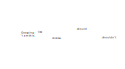
\includegraphics[width=\linewidth+18mm]{./manuscript/tex/diagrams/grasping-turbulence.pdf}

\smallskip

{\footnotesize
Turbulence in obstructed water flow.
The formation of vortices is similar to how grasping 'I am' in the mind
causes one to be stuck in a back-and-forth motion between opposite positions.
Fluid simulation by Amanda Ghassaei (\href{http://apps.amandaghassaei.com/VortexShedding/}{apps.amandaghassaei.com}).
\par}
\end{figure}

\clearpage

\section{Threads}

\keywords{suttas as literature}

\noindent In the days of the Buddha, one form of literature was the
\emph{sutta}, which means a thread of discourse. \emph{Suttas} may
include prose and verse, and were intended to be memorized through
recitation. The community of monks would compose a \emph{sutta} after a
significant event, such as a discussion or formal a teaching, to give
the story a formal presentation in which they would memorize it. The
Buddha certainly encouraged them to do so:

\begin{quote}
Thus you should train yourselves: `We will listen when discourses that
are words of the Tathāgata---deep, deep in their meaning, transcendent,
connected with emptiness---are being recited. We will lend ear, will set
our hearts on knowing them, will regard these teachings as worth
grasping \& mastering.'

\bigskip

\quoteRef{%

\href{https://www.dhammatalks.org/suttas/SN/SN20_7.html}{SN 20.7}, The
Peg

}
\end{quote}

Today, books, articles and blog posts fulfil a similar function, to
distribute curated information. These modern media, when bringing their
best form, hold up the canonical \emph{suttas} as their example. The
monks of the early years delivered their message to us through these
threads, and their efforts have become part of our conversation with
those we meet today, just as our written works will speak to those in
the future who we will never meet.

\clearpage

\keywords{social media, selection bias, Instagram Effect}

In today's social media the clear understanding of the message is
distorted by what is called `the Instagram effect', which is a selection
bias to show only our best and most positive side, and filter out the
negative one, which is nonetheless just as real and necessary for
complete understanding.

This influence is not negligible. Medical studies have already started
discussing a related form of depression and obsessive behaviour called
`Snapchat Dysmorphia'.\footnote{\href{https://www.ncbi.nlm.nih.gov/pmc/articles/PMC5933578/}{Is
  ``Snapchat Dysmorphia'' a Real Issue? (ncbi.nlm.nih.gov)}} In these
cases a given person seeks cosmetic surgery to look more like the
smiling photos they see in the application.

The automatic filters of the app edit every picture to be more
attractive, and if we repeatedly see our bodies shown to us (by the
application) as a nearly flawless image, \emph{that} becomes our mental
self-image, and the unfiltered image we see in the mirror seems wrong to
us.

One might consider a similar Instagram Effect in published articles
about meditation experiences. The author has a point to explain, and
they select a mix of personal experiences, opinions, and supporting
explanations from other authors.

The author may write truthfully and try to avoid selection bias, but
subtle, unconscious forms of self-filtering keep operating. The world of
the written text is always a constructed reality. Nonetheless, when it
succeeds in its goal, in the well-chosen words we recognize our own
experience.

\clearpage

\keywords{our mental images as role models}

The meditator who lives in our head is like a character in a poem, or
the hero in a myth. Our heroes are wiser and stronger than we are, so
that when we are feeling lost and weak, they can give us faith and
advice. They can have unshakeable peace, so that when we are feeling
awful, we are able to endure and wait until the difficulty ends.

Such mental images are, however, just that, and shouldn't be mistaken
for a real person. They are valuable sources for guiding ourselves,
their narrative description helps us to figure out what to do by showing
where we are in a bigger picture.

The role of a mental image is not to determine what we \emph{should
become}. When we relate to perceptions and ideals like that, we are
going to feel conflicted and inadequate, because the real circumstances
of our life are far more complex, rich with ambiguous, shifting
boundaries, and are not like the simplified, static reality of a mental
image. Mental images are tools for explanation. They are \emph{ways of
seeing} the world, and are examples of acting correctly in a given type
of world.

\clearpage

\section{Assumptions}

\keywords{mind and the world, mode of attention, actions and beliefs}

\noindent We may remember the verse in the Dhammapada which points out
that the world of our experiences is not independent of us:

\begin{quote}
Mind precedes all states of being: they are led by the mind, made by the
mind.

\emph{Manopubbaṅgamā dhammā, manoseṭṭhā, manomayā.}

\bigskip

\quoteRef{%

\href{https://suttacentral.net/dhp1-20/pli/ms}{Dhp 1}

}
\end{quote}

Does that mean that we are creating imaginary problems for ourselves?

We may start investigating by asking, `Can the subject experience
suffering?' Living beings can suffer, but a cultural idea or self-made
story cannot suffer, even while \emph{we are}. It changes our attitude
if the subject of our concern only exists as a story and not as a living
being. Such insentient stories include the narratives we have around
institutions, nations, money, fame, or other social fabrications.

Next, a quick moral safety test: `Would a wise person praise or
criticize doing this?'

Further on, bringing our view to the surface: `What assumption creates
this stress and pressure? What is the motivation for doing this? Without
what, would this have no significance?'

We can reveal such unconscious motivations by looking at our present
actions and choices. What we choose to do now expresses what we believe
in, the assumptions we have accepted in the past.

`Why am I choosing to do this, here? Where does this action come from
and where does it lead?'

The underlying factors for our actions may come, for example, from the
habitual conditioning of our environment. We may have not expressed in
thought why we do what we do, but have felt \emph{the results being
expressed on us}, whether good or bad.

Starting the investigation with a closer look at our actions and
\emph{then} asking about the thoughts motivating them is a productive
method. In our inner chit-chat we tell all sorts of contradictory things
to ourselves, but our actions give clear points of reference.

\keywords{the best place to learn, reversing assumptions}

The associated feeling might be awful, but if we treat it as sign to
turn toward the mind and investigate it, our approach will stay
practical and productive. `If I am here anyway, what can I learn from
this?'

We find access to our assumptions through uncovering our unconscious
motivations. Once we can express an assumption clearly, we gain the
freedom to reverse it, or drop it.

We may ask, `Does it help in this situation, if I reverse my
assumptions?' Perhaps looking at it in the opposite way is exactly what
is we needed either for peace of mind, or for dropping the issue as if
it never existed. Either way, we are not acting out of compulsion: we
are free to either let it go or \emph{choose} to follow it through.

\clearpage

\section{After the Storm}

\keywords{happiness and accomplishments}

\noindent Meditation guides say, `return to the present moment', but it
doesn't mean that you must like everything you find there. The point is
that this is the only place where you can live. If you are happy, you
are not happy in the future, but in the present. If you are suffering,
you can't understand it in the future, only in the present. In some
situations, no amount of brainy self-talk is going to make it better, it
is best to call it the way it is, and wait out the storm like a stoic.
Conflict is genuinely stressful, separation from what we love is sad,
and being alive always ends with the tragedy of our own death.

We tend to anticipate success, and we expect our hard work to be
justified in the future. Examine that moment of accomplishment, what do
you experience? There may be some emotional elevation -- surprise, joy,
exhilaration, relief -- then everything is back to the ordinary level.
The destination turns out not to be the deliverance we thought it would
be. If we were intensely focused to get there, we might not even
remember anything from the journey, and wonder where did all the time
go. We can be so intent on being productive, that we waste our chance to
live.

Contemplating death holds up a truthful, if somewhat scary, mirror to
our values. `If I were to die tonight, would I be happy to remember
living as I am living today?' This question can stir up more from the
deep recesses of the psyche than we wish for. I remember a time when my
response the word `happy' was exclusively anger and self-aversion.

\clearpage

\keywords{values, being busy, Hedonic Treadmill, burnout, contentment}

The term `Hedonic Treadmill' describes the adaptive process in which
each new achievement becomes the new norm in our psyche, and we feel
less and less emotional impact after succeeding at our goals. Like on a
treadmill, no matter how hard one tries to increase one's happiness by
pushing toward the next successful step, one still remains in the same
place. We spend our life travelling on the journey, not hanging out in
the destination. If we look closer, even the idea of any destination
evaporates, like when you fly into a cloud. `I thought I saw it right
ahead, but now that I'm here, I can't see it.'

Despite this, we seem to continue thinking that being busy, productive
and efficient, is somehow going to save us. When one project is
finished, we can feel that we \emph{need} another one because being busy
is the only way of existence we know.

\enlargethispage*{2\baselineskip}

The wise men of old repeat their message about contentment, but it seems
that we have to suffer the pain of burnout before we comprehend what the
problem is.

Bertrand Russell gives a diagnoses, `One of the symptoms of an
approaching nervous breakdown is the belief that one's work is terribly
important.'\footnote{\href{https://www.goodreads.com/book/show/51783.The_Conquest_of_Happiness}{The
  Conquest of Happiness by Bertrand Russell}} Henry D. Thoreau writes in
his cabin by Walden Pond, `It is hard to have a Southern overseer; it is
worse to have a Northern one; but worst of all when you are the
slave-driver of yourself.'\footnote{\href{https://www.goodreads.com/book/show/16902.Walden}{Walden
  by Henry David Thoreau}}

\clearpage
\figurepagelayout

\begin{figure}[h]
\caption{Achievements and the Hedonic Tredmill}\label{fig-hedonic-treadmill}

\centering

\includegraphics[width=90mm]{./manuscript/tex/diagrams/hedonic-treadmill-stairs.pdf}

\bigskip

\begin{minipage}{0.8\linewidth}
\centering\footnotesize

The Hedonic Treadmill is the tendency for new achievements to be adopted as a modified, \emph{normal} baseline,
and for our level of happiness to return to the same level as before.
After one desire is satisfied, the conditioned craving seeks a new state.

\bigskip

The person on the Penrose Stairs thinks that
they are getting further and higher.
From our outside perspective,
we see that they are merely returning to the same level as before.

\bigskip

Recall the definition of Noble Truth of the Origin of Suffering:
`It is this craving which leads to renewed existence,
 accompanied by delight and lust, seeking delight here and there;
 that is, craving for sensual pleasures, craving for existence,
 craving for extermination.'
(\href{https://suttacentral.net/sn56.11/en/bodhi}{SN 56.11})

\end{minipage}

\end{figure}

\clearpage
\normalpagelayout

What if you practice \emph{being free}, instead of practising \emph{to
become free}? The system of gradual training described by the Buddha --
while encouraging us to make diligent effort in our practice -- starts
with blameless happiness in the present, born of contentment through
moral- and sense-restraint.

\begin{quote}
{[}\ldots{]} they practice restraint, protecting the faculty of mind,
and achieving its restraint. When they have this noble sense restraint,
they experience an unsullied bliss inside themselves.

\bigskip

\quoteRef{%

\href{https://suttacentral.net/mn38}{MN 38}, The Longer Discourse on the
Ending of Craving

}
\end{quote}

\keywords{self-aversion, self-criticism, labyrinth of mirrors}

It is easy to over-correct being busy, and swing to the other extreme:
`I've had enough! I'm just going to quit everything!' This might seem
``logical'' but, being driven by aversion, we continue to suffer. For
many of us, it is easy to be critical of ourselves, and we diligently
practice it with conviction to prove ourselves wrong, as if
self-aversion was a virtue.

`I am feeling awful! A \emph{real} meditator would never feel like this.
I must be doing something wrong.' A whole identity can be built around
this, a ceaseless internal monologue which always responds with
complaints and self-aversion. One can live like this for decades, and it
becomes the baseline by which we recognize ourself. `If I wasn't feeling
angry, I wouldn't even know who I was.'

It is like being stuck in a labyrinth of mirrors: everywhere you look,
you only see yourself. The key to escape is to find a crack in the
mirrors, and recognize change: the feelings of being driven, and the
motivations of anxiety and anger which we thought were constant are, in
reality, changing all the time -- breaking up and reforming. This
labyrinth has been made by the mind, and what it has created is empty of
self. It cannot be what we truly are.

Doubtless, we can find a persuasive logic in our self-defeating
ideations, and our reasoning for being critical can be completely
reasonable! Psychologists say that the most difficult patients are the
ones who intelligently defend and justify their own bad habits. We can
be so clever that there is absolutely no way to be happy \ldots{} and we
can prove it! Can you recall ever playing the role of such a miserable
philosopher?

But we do not necessarily experience immediate relief when our
self-reflection reveals to us the emptiness of what we have been
pursuing. Anger, despair\footnote{The Buddha compares dealing with anger
  and despair to walking along a path close to a deep drop-off.
  (\href{https://suttacentral.net/sn22.84}{SN 22.84}, With Tissa)} and
sadness can be our first reaction, generating thoughts of self-aversion.
We purify the mind with the mind: These mind states are not reliable,
they shut down our intelligence, and who wants that? So we let go.

\keywords{patient endurance, gratitude, no hurry}

Patient endurance is an underappreciated virtue, but often, all we need
is to remember to wait: the dramatic rain and thunder of turbulent
mental states will run themselves out.

When the sense of gratitude appears, it is a sign like the rainbow after
a storm. It accompanies wholesome mental states, and we can
intelligently see the situation from more than one angle. This is a good
base from which we can build useful thoughts about what to do next.
Sometimes, the best thing to do is to simplify and turn away from
certain habits and values. Other times, our view has changed and we
might wish to keep up what we have been doing, but leaving the big hurry
behind. We continue for the sake of living it, not waiting for some kind
of elevated mental state in the future.

\begin{quote}
One should not revive the past\\
Nor speculate on what's to come;\\
The past is left behind,\\
The future is unrealized.

\bigskip

\quoteRef{%

\href{https://suttacentral.net/mn131}{MN 131}, One Fine Night

}
\end{quote}

\section{Humour and Irony}

\keywords{opinions, changing perspectives, noticing what is pleasant}

\noindent There are morose, dark moods which are like sand-traps of
logic, made by ourselves. The more we think about them, the deeper we
sink in them.

Humour and irony are funny because they show the situation from
unexpected and odd angles. If the logical path straight ahead is
blocked, why not try the sideways track where the fox goes? A joke
wouldn't be funny if it was logical and reasonable. Humour and irony,
directed toward ourselves, are good friends when it seems that we can't
escape the suffering of our thoughts.

What makes the old and wise men \emph{wise}? Medical studies\footnote{\href{https://www.researchgate.net/publication/258190619_Aging_irony_and_wisdom_On_the_narrative_psychology_of_later_life}{Aging,
  irony, and wisdom, William Randall (researchgate.net)}} have
investigated the various attitudes of senior citizens, and found that an
inclination toward self-directed humour and irony (i.e. being able to
laugh at oneself) was helpful to face the significant challenges of
ageing and maintain mental balance and a positive outlook on life.

One of their key observations is that humour and irony develop our
ability to see ourselves from multiple viewpoints. We can fill the role
of the accurate historian and the jesting comedian at the same time.
Hence we are able to see events from multiple narrative angles and not
be caught in a single story. The frame of the narrative we see ourselves
in remains open as we move toward a positive future. The limits of our
being don't necessarily mean the end of the story, and we don't have to
go far to find good laugh: in the absurd corners of life, there is
always a joke to tell.

It can be rude to joke about somebody else's bad situation, but who is
going to get upset over your humorous comments about yourself? If you
feel awful, how about an awful joke? This trip is so bad that it's good,
and the tickets are free. `What am I? An animated skeleton in a skin-bag
with clothes on, standing here with a fabulous hair-cut, and I can prove
the logic of \emph{my important} opinions.' What's not to laugh at?

\enlargethispage*{\baselineskip}

We say that in meditation we observe our own mental habits, but
sometimes we practise this with a critical bias: we observe the
\emph{bad mental habits}, while we don't notice the good ones. It is
possible to become so good at ignoring pleasant mind states that one
genuinely believes happiness only exists for other people. When
something good happens and you feel happy, stop and notice it, `Hey,
this is nice.' This increases our capacity to recognize and experience
such mental states in the future. Who will notice it if you don't?

\section{Expectations}

\keywords{symbol of Buddha statues, changing predictions, relinquishment}

\noindent We might look at a Buddha statue and expect ourself to
meditate in the same perfect posture without moving, like the Buddha.
But in this case we have missed the message of the statue, which points
to inner qualities rather than external signs.

A Buddha statue is not a depiction of the historical \emph{Siddhattha
Gotama} Buddha who lived in the 5th century BC. We don't have a statue
of him made during his lifetime. We know from the \emph{suttas} that he
was normal height and good-looking, but instructed the monks to not
focus on his physical appearance, bot on the Dhamma, the truths of the
mind instead.

He taught them that even if a monk were grabbing hold of the corner of
his robe, but if they didn't see the Dhamma, they would not see the
Buddha.\footnote{\href{https://suttacentral.net/iti92}{Iti 92}, The
  Corner of the Cloak} The first Buddha statues were made four or five
hundred years after his death by Greeks in the Gandhara region of
Afghanistan. Buddha statues represent the wisdom and serenity of the
awakened mind, expressed in the human form.

They are beautiful to look at, but nobody is going to become a Buddha
statue, just like you can't become the photo of the perfect meditator,
or the hero in lyric poem. They do offer advice, but the advice can't
orient us when taken rigidly. We should apply the advice by taking our
inner experience and the present situation into account. This way we
return to the awareness which awakens to the truth and overcomes
obstacles. The practice of virtue, and the trust in the examples of
skilful teachers is a strong foundation. We can wish ourselves well,
while still admitting that we feel awful, when that's how it is.

Expectations are a prediction of the expected value of a result, they
estimate the outcome of our situation. Meanwhile, every factor which
goes into that prediction is changing. We have to allow the prediction
to change, our expectations of our mental experience must keep changing
according to where we are now. Having expectations is not a problem, but
if we attach to a particular outcome which we believe to be `the real
one', this becomes a hindrance. It turns out that if we invest in future
emotional states as the basis for our happiness, the result will be
disappointment.

\enlargethispage*{\baselineskip}

The \emph{ānāpānasati} breathing technique taught by the Buddha has
sixteen steps. The first is knowing whether the breath is long or short.
But what is the last step? We might wonder, `What could be that exalted
mind state which we will reach?' Mindfulness meditation on the
breathing, after contemplation of the body, feelings, and mental states,
follows contemplating the natural truths, of which the last step is:

\begin{quote}
One trains thus: `I shall breathe in contemplating relinquishment'. One
trains thus: `I shall breathe out contemplating relinquishment'.

\bigskip

\quoteRef{%

\href{https://suttacentral.net/mn118}{MN 118}, Mindfulness of Breathing

}
\end{quote}

The practice of the Eightfold Noble Path is not about accumulating, but
about transforming our values through insight into the experience of
changing conditions. At the end we relinquish the conditions, like
putting down a burden and not carrying it any further. This includes all
that we take to be `me and mine'. Anyway, how long can we really hold
onto anything?

\keywords{real practitioner, Impostor Syndrome}

Reflection and cultivation opens up a wider field of view where
opposites can exist in complex relationships. In the contrasting
approach, we exalt the judgmental and comparing mind, and this limits
our scope. Such a perspective wants to sort things into neat, mutually
exclusive abstract categories, which leads to mistrust and harm. We
start losing faith, not believing ourselves to be `real' practitioners,
and others don't seem to be credible ones either. The result is that we
can't learn from ourselves, and we can't accept anyone to teach us
either. This doubt is blinding and paralysing, it feels like we can't do
anything. The problem is that our expectations are too narrowly focused.

It's not that there are no problems and difficulties. Explaining to
ourselves that `pain is not painful' is not a meditation technique
taught by the Buddha. But we shouldn't assume that we should be like
mythological ideals. Meditation is not a button to control mental
states. It is cultivating awareness, so that mental states don't control
us.

\section{Calibrating Emotions}

\enlargethispage*{\baselineskip}

\keywords{learning emotions, variation is the norm, disappointment, saññā and saṅkhāra}

\noindent When we talk about emotions to each other, we often explain
their mechanism roughly as a `neural circuit', or a region in the brain
which gets activated in a certain situation. According to this story,
some brain areas are wired from birth to produce given emotions, and
they make us feel fear, love, anger or disgust.

But then how do we explain it when a person without an \emph{amygdala}
still experiences fear? The \emph{amygdala} is typically seen
responsible for that emotion.

Or how about more refined categories?

The Japanese `\emph{mono no aware}' means a sadness over transience and
the beauty found in that, are the Japanese born with such a neural
circuit? By the description, you might recognize the feeling, if you
have seen Japanese movies it might even be familiar, and now, fitting a
verbal expression on it, it gets easier and easier to feel it.

Other cultures find the western emotions strange, for example the Utka
Eskimos, who have no direct equivalent of the concept of `anger.' Or the
Tahitians, who have no concept of `sadness.'

Medical research informs us that no particular emotion has a built-in
`brain-circuit' from birth.\footnote{\href{https://www.goodreads.com/book/show/23719305-how-emotions-are-made}{How
  Emotions Are Made: The Secret Life of the Brain by Lisa Feldman
  Barrett}, Theory of Constructed Emotion} It is not the given emotion
that is fundamental, but our ability to recognize patterns of loss and
reward, to \emph{learn emotion concepts} from other people, and to
recognize them in a new situation in the future.

In any given situation, the brain recognizes if an earlier experience
\emph{in a similar context like this} was rewarding or not. This becomes
easier over time if we have learnt to associate an emotion concept with
it, becoming a spontaneously automatic feeling.

The instances of an emotion category are variable: `fear of a tiger' is
different from `fear of an exam', which are learned and adaptive
predictions. They fit only to some extent, like a person may fit a
stereotype, but no person is a 100\% example of every feature of the
stereotype.

Our brain evaluates the present based on the past, and according to
whether good or bad can be expected, there is a response we feel
throughout the body, and we construct an instance an emotion from it
based on our concepts.

\keywords{emotions are categories, not distinct mental object, learning emotions, what is wrong with me}

In the classical model of emotion -- which we are accustomed to in
everyday discussion -- we treat emotions as distinct mental objects. The
idea is that an emotion has clear attributes that any two mentally
healthy people should agree on.

However, while they were studying the brain in action, it became
apparent to the scientists that this cannot be the case. As they
conducted more and more studies, the evidence continued to contradict
this view.

When people undertook physical and psychological tests about the
emotions they experienced, the results had great variation between
individuals. There were no universally distinct, clear markers, or
`fingerprints' to identify any given emotion. Rather, the
\emph{variation was the norm} in both people's emotional experiences,
the meaning and function of those emotions, and their corresponding
physical reactions.

The scientists found that our body and brain \emph{learns} emotion
categories through a process of conditioning perceptions. From our
culture, the other people we live with (socially conditioned emotions);
from biological needs (bodily conditioned \textasciitilde); or from our
personal history, such as long-time habits, significant events and our
memories.

This also relates to how one person might not understand, or not even
recognize, the emotions of another. For example think of the culture
shock when visiting a distant country: an emotion such as `love' has a
variety of expressions, contexts and underlying assumptions which were
not part of our earlier emotion category of `love'. It can take a while
to pick up the new signs and meanings until we can feel the subtle
differences, and we can reliably recognize the signs in others.

Ask yourself, how do you know that you are feeling a particular emotion
such as \emph{metta} (loving-kindness) or \emph{sukha} (happiness)? The
model we use for our understanding of emotions influences what we expect
to happen in our meditation practice. If we think of emotions as
distinct things, as though they were external objects which we wish to
reproduce, or have access to, then we can easily feel `this is not it, I
don't know what's wrong with me'.

Since \emph{variation is the norm}, our experience will probably differ
from other people's. Individual meditation experiences are as varied as
the individuals. A given instance of an emotion can be expected to vary
from the generalized idea. It is important to rely on knowing \emph{our}
mind states and feelings, instead of trying to reproduce external
descriptions.

Our freedom extends to learning and constructing emotions we never heard
of before. We rely on mindfulness to perceive our experience, we
self-train the concept, and establish the conditions for the emotion to
arise.

Using the terms of the Five Khandhas, we would say that perceptions
(\emph{saññā}) and mental conditioning (\emph{saṅkhāra}) influence each
other and establish patterns of experiences, which we learn to identify
as a present instance of a broader, abstract emotion category.

We start with reading the external description and we turn it into an
inner experience through reflection and daily actions. Knowing our
experience is the reference point. Over time, the new experiences become
familiar to us and they arise without effort.

\keywords{emotions as predictions, culture shock, adjusting expectations}

The brain is constantly receiving signals from the nervous system, and
based on what it has learned, it tries to predict whether the present
situation is going to mean energy input or energy expense for the body.

The brain responds by preparing your body, such as increasing or
decreasing the heart rate, starting or stopping the production of
certain hormones. We experience this bodily reaction, and if earlier we
learnt an emotion category which suits this, we feel an instance of that
emotion: fear of danger, excitement in anticipation of immediate reward,
or euphoric happiness.

This explains culture shock: if you have grown up in a different
culture, you've learnt different emotion categories, and when travelling
to a distant country, the emotional world of the people living there can
be unfamiliar to you.

We tend to believe that our experience is like the view when we look out
a window. One `looks onto their experience', and sees what is going on.

It turns out that the picture is rather more incomplete than we think,
when we take into consideration how the senses and the nervous system
work. The brain doesn't have much information to work with, so it has to
guess at what is happening from simple signals, hints about what the
rich world outside of itself might be like.

The brain can't see much: it's sitting in the skull, which is, in
effect, just a dark box. Bodily fluids, chemicals and nerve signals
carry messages into this box. The messages come from other systems in
the body, which are themselves noisy and sometimes conflict with each
other. From this clutter, the brain has to generate a perception of the
place where we are, guess what is happening to us, predict what is
likely to happen in the next minute or so, and produce a response which
is hopefully going to help us survive, or even lead to happiness. It has
to do all this, from inside a dark box, based on a few noisy and limited
signals.

\clearpage

What am I then? An animated skeleton, and my head is a dark box? Well,
that does explain a lot of confusion. Is it a wonder that my predictions
are a bit off, and need constant adjusting? What I experience as reality
is ongoing guesswork, changing by the second.

`Happiness equals reality minus expectations' -- a memorable phrase by
Tom Magliozzi. These days, our expectations are so high. We receive
updates from social media apps, we read web articles, and each time they
influence our view of how we are, and how the world is around us. They
show us perfect, determined, or outrageous images of other people. Since
we don't meet these people face-to-face, we don't see the real
background of their lives, and this exaggerates our expectations. It
trains the brain again and again to expect these artificial
presentations, like an expectation machine on overdrive. We don't even
notice the distorted self-conditioning, but we are disappointed and
exhausted, which leads to ceaseless dissatisfaction.

\keywords{simplicity, impermanence, self-reflection, values}

We have the ability to calibrate the `expectation machine' through the
balancing effect of conscious reflection and reasoning. `What is the
most important today? What do I need for this one day?' When you
simplify the answer down to the essentials, it's not that much. Food,
clothes, shelter, medicine, supportive companions and perhaps something
to do toward a worthwhile goal.

The average day is probably more messy, and doesn't hold to this
abstract, pure simplicity, but this exercise is only for recognizing the
baseline. If simple is enough, then it won't be a problem to be able to
do more, or have access to more, while contentment remains our baseline.
Ambition is not the problem, but hyping up our expectations blocks its
application.

Expectations are necessary to follow a given direction in the world, but
not understanding them, they become obstructions in the heart.
Expectations and emotions are of the nature to arise, twist, flip-flop
and then turn around. Let them pass on by, like leaves in the water next
to a boat. Bad ones are not that bad and good ones are not that sure.
Knowing their changing nature, we don't take them so seriously and don't
get stuck on them, as a boat shouldn't get stuck on some leaves.

\begin{quote}
Whether it be pleasant or painful\\
Along with the neutral,\\
Either internal or external,\\
Whatever feeling there is:\\
Knowing them, `This is suffering,\\
deceitful and disintegrating,'\\
Coming in contact again and again,\\
seeing their fall,\\
One loses one's passion for them.

\bigskip

\quoteRef{%

\href{https://suttacentral.net/sn36.2}{SN 36.2}, Pleasure

}
\end{quote}

\clearpage

\section{Happiness as Flourishing}

\keywords{meanings of happiness, results, day-by-day practice, death, contentment}

\noindent Our modern Western culture often presents happiness as a
particular feeling, or as a certain circumstance in life which we are
supposed to arrive at. We pass on our culture through discussion with
one another. Our way of talking about happiness tends to treat it as an
outcome, as an event in the future, or as a certain state of being. This
seems to be a recently developed trend, and not necessarily a helpful
one.

Traditionally, we view the ancient Greeks as one of the most influential
societies in the formation of our Western values. Aristotle (384-322 BC)
is one of these influential thinkers, and today we are still reading and
referencing his writings which survived the ages. In these texts, he
investigates the question of happiness in great detail.\footnote{\href{https://plato.stanford.edu/entries/aristotle-ethics/}{Aristotle's
  Ethics (plato.stanford.edu)}} He was concerned with what happiness
was, and with how to live a happy life, but, unlike us moderns, he did
not see it as a particular result or circumstance.

The Greek word he used for happiness is \emph{eudaimonia}, and can be
translated as `human flourishing, prosperity.' He saw it manifesting as
a continuously active process which we practice day by day, rather than
an eventual outcome in the future. He describes the practice of
happiness as being based on moral virtue and a truthful view of one's
life from birth, growing up, old age, and including the tragedy of one's
own death.

\enlargethispage*{2\baselineskip}

This direct view of virtue and mortality puts things in order: it gives
us a wide perspective in which happiness is founded in wholesome mental
qualities, and we look beyond ourselves to give lasting meaning to it.

Training our expectations in this way, the practice of happiness is a
complete whole every day. We learn to be with the struggle when that's
how it is, applying our best abilities in virtuous ways, and at the end
of each day, we can look back with contentment.

If the field of `happiness research' in psychology, Daniel Kahneman and
his team have conducted interviews asking people to recall the episodes
of the previous day and to later answer questions about them.\footnote{\href{https://www.goodreads.com/book/show/11468377-thinking-fast-and-slow}{Thinking,
  Fast and Slow by Daniel Kahneman}, Day Reconstruction Method} The
evaluation confirmed that attention and recurring thoughts are the
dominant factors in whether one feels happy or depressed. While the
volunteers were going through a variety of everyday situations, how they
felt was determined not by where they were and what they were doing, but
by what they were thinking about at the time.

\keywords{deathbed regrets, life as a unit of time, hierarchy of needs, self-actualization, self-transcendence}

\enlargethispage*{3\baselineskip}

But it surprised them to find that when people spoke about what kind of
day they had, they didn't talk about happiness as a good feeling, but
rather they reflected on social experiences, friends and relatives, who
they met and what they did together, and on whether they felt satisfied
with their life or not.

All this makes sense when we examine our experience: the perspective,
the frame through which we see the world orients us, while the content
of the frame continues to change. The hungry person sees the world in
terms of food, and where to get it. A person in an ambitious mood
focuses on `what I can do' and `how good I am'. A person considering the
limited time of his personal existence, tends to turn toward values
which are self-transcendent. Rather than focusing on experiences created
by the self, one turns to timeless qualities apparent here and now.

It was a discovery for me when I was listening to an
interview,\footnote{\href{https://www.samharris.org/podcasts/making-sense-episodes/209-a-good-life}{A
  Good Life: A Conversation with Scott Barry Kaufman}} and heard the
psychologists discuss a new addition to Abraham Maslow's hierarchy of
needs. This is usually pictured as a pyramid starting with the need for
food and water at the bottom, and ending with self-actualization
elevated to the pinnacle. This seemed to be a rather ego-centric way of
thinking about happiness.

The psychologists recently re-discovered Maslow's late
writings,\footnote{\href{https://bigthink.com/neuropsych/maslow-self-transcendence/}{Maslow's
  forgotten pinnacle: Self-transcendence (bigthink.com)}} and found that
toward the end of his life, he felt conflicted about his system of the
hierarchy of values: he was going to die, fundamental parts of his needs
(e.g. survival) were lacking, hence he should be miserable, but instead,
he felt relief and states happiness which he called `peak experiences':

\begin{quote}
Feelings of limitless horizons opening up to the vision, the feeling of
being simultaneously more powerful and also more helpless than one ever
was before, the feeling of great ecstasy and wonder and awe, the loss of
placing in time and space with, finally, the conviction that something
extremely important and valuable had happened, so that the subject is to
some extent transformed and strengthened even in his daily life by such
experiences.
\end{quote}

\clearpage
\figurepagelayout

\begin{figure}[h]
\caption{Hierarchy of needs, self-transcendental values}\label{fig-self-transcendental}
\bigskip
\includegraphics[width=\linewidth]{./manuscript/tex/diagrams/self-transcendental-values.pdf}
\end{figure}

\clearpage
\normalpagelayout

Maslow appended another level to his hierarchy of needs above
self-actualization: \emph{self-transcendence}. Examples include: not
holding onto perfection, not fixating on one's opinions, giving up the
need for certainty, giving up the attachment to one's past and letting
go of the fear of death.

`Self-transcendence' sounds like something for a Buddha, but since we
are suffering from our attachments to one thing or another, it turns out
to be a basic \emph{need} for all of us.

Holding onto what we think we are creates the very limits which we
struggle with. We want to expand our horizon but we are held back by
grasping an identity. When that identity turns out to be an empty void,
we urgently need help. Think of the day-to-day struggles: being
conflicted over opinions, stressed out about our abilities, anxious due
to unexpected changes, lamenting past tragedies. A self-transcendent
perspective is necessary to get over ourself.

\enlargethispage*{3\baselineskip}

Still, we do keep the score on how things are going for us, don't we?
Wholesome conditions are our supports. This is the time and place where
we live, not any other: \emph{memento vivere}, remember to live. We know
if our efforts are aligned with our core values or not, even though we
can get distracted with things we didn't intend to spend so much time
on.

I remember how it shook me up when I read in a description by a
nurse,\footnote{\href{https://bronnieware.com/blog/regrets-of-the-dying/}{Regrets
  of the Dying (bronnieware.com)}} that some of the most common deathbed
regrets included working too hard and losing touch with old friends.
Life is a unit of time with a beginning and an end, and we should treat
it as such.

\clearpage

\keywords{\emph{memento mori}, \emph{memento vivere}, \emph{amor fati}, \emph{saṃvega}, \emph{pasāda}}

If tuning the mind to a comfortable numbness is `tranquillizing
ourselves with the trivial',\footnote{A phrase used by Søren Kierkegaard
  in The Sickness Unto Death} then recollecting death (\emph{memento
mori}) is a dose of anti-tranquillizer. Since the time is limited, we
recollect the urgency to live (\emph{memento vivere}) and do what must
be done before it's too late. This motivates us to find the courage to
be true to ourselves and turn toward the situation we are living in
(\emph{amor fati}), not waiting for some place and time we imagine in
the future. In the Pali language of the Buddhist \emph{suttas},
\emph{saṃvega} refers to the sense of spiritual urgency, while
\emph{pasāda} expresses the serenity of having confidence in the Path
and its practice.

Reading about deathbed regrets was a timely reminder for me to think
about the urgency I felt about completing projects (which come and go by
the month), and not losing the opportunity of spending quality time with
long-time companions.

Reflecting on life as a single unit of time includes being born, growing
up, growing old and dying. Remembering our mortality this way puts our
values back in line with the facts of nature. We can give ourselves some
time to dwell where we are, and appreciate it before it's over. We seem
to understand the fleeting nature of good and bad feelings when we
compare them to the importance of our golden relationships.

\clearpage

Remember that we wish ourself well-being and happiness, and that we wish
our family and friends happiness in their life. Consciously recollecting
moral virtues builds mental resilience and self-respect. We can
acknowledge ourselves: `That was a good thing to do. I've done that
well.' Or, we see it in others, such as in teachers, role models, and
friends.

It develops gladness and appreciation of what is good in other people as
we share in their successes. There is a wellspring of happiness in
cultivating the face-to-face companionship of friends whom with we
mutually feel glad at our successes in life. We can use humour to ease
up a bad mood, and complete the next step forward.

The present is change itself. We bring that experience into awareness
and contemplate the body, feelings, mind states and natural truths
following the refrain in the \emph{Satipaṭṭhāna Sutta}:

\begin{quote}
\ldots{} One dwells contemplating its nature of arising, or one dwells
contemplating its nature of ceasing, or one dwells contemplating its
nature of both arising and ceasing. \ldots{} And one dwells independent,
not clinging to anything in the world.

\bigskip

\quoteRef{%

\href{https://suttacentral.net/mn10}{MN 10}, Mindfulness Meditation

}
\end{quote}

\chapter{Why}

\section{Doubt and Faith}

\keywords{compulsive thoughts, orientation of views, unexpected changes}

\noindent Sometimes we are interested in meditation in order to deal
with a disturbing or painful experience. We know something is wrong and
we can't shake it off. Or it could be a sense of feeling lost, where
nothing makes sense: such feelings keep returning, they don't let
themselves be ignored. Instead of answers, only the questions keep going
round and round: `Why does it have to be like this? What should I do,
and why? What's the point?'

Even in such confusion, merely acknowledging the state of our inner
chaos to ourselves already starts to provide some order and orientation.

\enlargethispage*{\baselineskip}

It is like driving on a road cluttered with trash. Slowing down to look
around is already much better than being blind to the dangerous clutter.
Our head is full of thoughts but only a few of them indicate reliable
directions, so we better examine them. Previously, we held a view that
things in our world were one way, but they have changed in a way we
didn't expect. It is not their fault, it is not our fault, but the
unexpected change is confusing, and we have to adjust our view.

Impermanence pulls the carpet out from under our feet, but at the same
time transforms our values, the qualities which we seek out as valuable
in our experiences. If we don't understand the change, it causes
confusion, followed by doubt. Even though we might know what we
\emph{should be doing}, we get stuck in the sense of doubt and
meaninglessness and we can't even begin.

\keywords{meaning, investigating what I believe, faith as fuel}

Why do you get up in the morning to do anything? Why does it matter at
all? If I keep asking `why' and dig into the layers of my constructed
self like this, the first layer reveals a matter of habit, `because this
is what I did yesterday'. Under that, the answers are formed out of
stories I tell myself about myself and the world I live in. Under that,
there is some degree of reasoning, philosophy and abstract ideas. Under
that, I am desperately trying to hold onto something solid, and I start
defending my ideas with personal memories and experiences (`because when
I was like this and this \ldots{}'), or I refer to famous names
(`because this and that teacher said \ldots{}').

Under that, I have to give up and confess that it is a matter of faith
and personal conviction. What I do is simply what I decide there and
then. At the end, I stand there and have to admit that I don't
\emph{know}, but I \emph{believe} that doing such-and-such makes sense.

Faith is not a fixed quality in the mind. We have the capacity to choose
credible statements which we perceive will guide us toward a greater
understanding and happiness. We can test any given belief by applying it
in practice and by observing the results, and we can then support or
abandon that belief accordingly.

I may review, investigate and update \emph{what I believe} about what
makes sense to me, but until my experience verifies it, my reasoning has
to be supported by faith. Otherwise, I will not make an effort in any
direction, and my life will be governed by blind habits and external
pressures.

Faith is the fuel for the virtues of resolve and energy. Later on, faith
will be reinforced by experiencing the results of practice, but without
fuel, our car doesn't even start.

\keywords{belief as a cause of action, trust in the teacher}

A belief creates a cause for an action. Without that belief, I don't
take that action. In the Buddhist perspective, there are two fundamental
beliefs:

\begin{enumerate}
\item
  A phenomena occurs when the sufficient causes for it are present; and
  it either does not occur, or it ceases, when the sufficient causes are
  absent.\footnote{\href{https://www.dhammatalks.org/suttas/SN/SN12_61.html}{SN
    12.61}, Uninstructed}
\item
  The Buddha completely understood the truth about the way things are,
  and thus freed himself from greed, hatred and delusion. Hence he is an
  excellent teacher of the way of practice.
\end{enumerate}

The Buddha gave us the instruction that each person should question,
ponder, and investigate the way things really are to understand it for
themselves. Nonetheless, how are we going to start? Without trust in the
teacher, we are lost in the tangle of our personal opinions and it is
unlikely that we are going to listen and learn anything new. The
tradition reminds us of this relation to faith when, before giving a
Dhamma talk, we start by chanting \emph{namo tassa} three times.

\begin{quote}
\emph{Namo tassa bhagavato arahato sammā-sambuddhassa}

Homage to the Blessed, Noble, and Perfectly Enlightened One.
\end{quote}

\keywords{doubt, wandering in a desert, grasping creates limits}

The Buddha compared doubt to being lost in a desert, wandering around
without water.\footnote{\href{https://suttacentral.net/dn2}{DN 2}, The
  Fruits of the Ascetic Life} Everything else is secondary: we can only
think about how to find water and escape the desert.

Or, we fantasize about how to comfortably numb the mind and not think
about anything at all, `tranquillizing oneself with the
trivial'\footnote{Søren Kierkegaard, `The Sickness Unto Death'} to
continue everything as normal. In doubt, it is not clear how we will
escape this situation, but we can start by acknowledging the aspiration
to be well and to live a happy life.

It is our natural human ability to overcome confusion and develop
long-term happiness in our lives. A long-term view has to include
changes to our situation, loss and tragedy. Stable happiness has to be
founded on a perspective which integrates impermanence.

In the \emph{suttas}, doubt appears both in the list of Five Hindrances,
and in the first three of the Ten Fetters, which are the ones that
obscure understanding the Four Noble Truths. When doubt gets personal,
there is no doubt that it leads to suffering. Figures
\ref{fig-leading-to-suffering} and \ref{fig-leading-to-cessation}
illustrate how we get into this mess, and how we can get out of it.

As a hindrance, doubt stops Right Effort, and stops developing the mind.
As a fetter, it compels us to keep looking for fixed certainties, and
thus ties us even tighter to our ideas about who we are.

We like the suggestion to develop our mind, but initially, we think this
means making sure who and what we are, getting more of what we need, or
changing ourselves to become something different.

`Who am I? What am I? What should I do? Is this the right thing? Or is
it something else?' This way of thinking is a trap, it goes round and
round with no way out. All these concerns are tied up with holding onto
some kind of identity which will again invite doubt. Until we realize
what is happening, we are caught in the cycle.

Even when we become successful, at the end of that becoming, it is going
to change according to its nature, and we find that our new identity is
also hollow, empty of real value, just as our previous idea of ourself.

Grasping at and holding onto what we think we are, being afraid to let
go: this is the obstruction. This creates the very limit we are
frustratedly running up against. Understanding freedom through letting
go doesn't come to us easily.

\cleartoverso
\figurepagelayout

\begin{figure}[h]
\vspace*{-10mm}%
\caption{Leading to Suffering}\label{fig-leading-to-suffering}

\centering

\includegraphics[width=\linewidth]{./manuscript/tex/diagrams/leading-to-suffering.pdf}

\end{figure}

\clearpage

\begin{figure}[h]
\vspace*{-10mm}%
\caption{Leading to Cessation}\label{fig-leading-to-cessation}

\centering

\includegraphics[width=\linewidth]{./manuscript/tex/diagrams/leading-to-cessation.pdf}

\end{figure}

\clearpage
\normalpagelayout

\section{Right View}

\keywords{returning to the beginning, observing thoughts}

\noindent Let's return to the breath and continue the meditation
practice. At the beginning of a session, start with the basics, simple
steps which guide the attention back to the familiar frame: the in- and
out breath, the body and its feelings. Observe what you are experiencing
as a process which is going through continuos change from one feeling
into another.

Every meditation session is a new beginning, we can't save the results
of the previous session and load in the knowledge. If we start thinking
we already know, say, if we have been practising this for years, this
results in a closed attitude which blocks even our earlier
understanding. Our experience from the past is only relevant when we
apply it to the present. The changing present keeps understanding fresh
and new.

`This thought, this feeling had a beginning, it is changing now, it will
cease and end. Can I wait and notice that cessation?' Contemplating
direct experience this way, the mind gives up its desire and fear
regarding particular states, and understands them as part of natural
processes. We are not reasoning to ourselves about what we think about
the mind, rather, as if taking a step back and watching it, we mindfully
experience the way it is.

\enlargethispage*{2\baselineskip}

This contemplation restores Right View, as if someone took an upside
down flower vase standing on its top, and put it upright again. When we
look, we understand which part of the vase is the top and which the
bottom. We crave and want to hold onto experiences that are always going
to change, doesn't that sound stressful? Fortunately the mistake is
avoidable.

\clearpage

\keywords{freedom around limitations, essentials, gratitude, flooded with good advice}

Right View finds space and freedom around the limitations and pressures
of life. At first, we might not see much open space, but contemplating
the essentials, we might notice that we don't need everything we can
think of. We can ask, `Do I have what I need for this single day?'

We can take stock of what we are using in our immediate environment --
clothing, food, shelter, medicine. Sometimes, others give them to us or
allow us to use them. At other times, we give them to others. `Do I know
how much is enough for today?' A sense of calmness returns when I
recollect them again, even though I might know these fact already.

Recollecting the simple things, that we have what we need to live this
day well, our attitude expresses itself in feelings of contentment and
gratitude for life. You don't have to ask for them and you can't create
them by will. We have to make space for them in our view, then they
arise on their own.

What's the great hurry for? A simple exercise is to stop and do nothing
for two minutes, not looking for entertainment and distraction. You can
watch the breath, but this is optional. Not rejecting boredom as a
mental state increases our focus and preserves energy.

The problem is not that we don't know enough. The bookshelves are
overflowing with good advice about `how to be happy'. If that's all we
need, where is the problem? If all it took was good advice, all of us
would have gotten enlightened long ago. We hear and read about all the
good things we should do and what sort of person we should be: one book
says we should be tough and fearless, while another says we should have
universal compassion. It is a special kind of suffering to read it all.

Or perhaps we need \emph{Nibbāna}? Is that the right idea? The meaning
of the word is `going cool', as in a fire ceasing to burn and growing
cool. A craving to `have it' means more fuel for the heat and burning of
becoming.

But \emph{Nibbāna} is the coolness of ceasing to burn with becoming, so
should we become this non-becoming? The thinking mind goes,
`\emph{What?!}' And that's not a wrong answer either: the teaching of
the Buddha points out that thinking and becoming are not sufficient
tools here. Any other state or thought, when we see ourselves in it,
will be as limiting as the previous one. We are not freed by
\emph{becoming} the right thing, but by recognizing that we can give up
the compulsion to continue becoming.

\clearpage
\figurepagelayout

\begin{figure}[h]
\caption{Experience, Becoming and the Deathless}\label{fig-experience-becoming-deathless}
\bigskip
\includegraphics[width=\linewidth]{./manuscript/tex/diagrams/experience-becoming-deathless.pdf}
\end{figure}

{\noindent\footnotesize
See also: Chapter 10, Birth, Decay and Death in The Buddha's Teaching: It's Essential\\ Meaning by R. G. de S. Wettimuny
\par}

% TODO: link to Wettimuny book

\clearpage
\normalpagelayout

\section{New Eyes}

\keywords{turning toward experience, intellectual knowledge, watching the senses}

\noindent We can turn a compulsive tendency into meditation practice by
asking, `How can I understand this experience?' This question directs us
to the noble attitude towards suffering described in the Four Noble
Truths: `Suffering should be understood.' Discard the opinions which
present themselves as answers, and keep returning to this open attitude
of knowing the present.

Both joy and sorrow are natural processes, but if we don't understand
them, we see one as a reward and the other as a punishment. Life never
seems to be fair and it always seems to be out of our control.

To open up our attitude for contemplation, we can at least imagine the
possibility that there is something here we can learn. A turning point
occurs when we are able to let go of being sure about our opinions and
can stop to investigate the experience itself.

Consider how narrow our attitude is when we start with the thought,
`I've seen this, I know this'. Perhaps this is true, but I notice that
when I try to use that intellectual knowledge to solve a problem, my
attention merely revolves around memories, thoughts and opinions. While
I am caught up in the past, the present experience escapes my attention.

The instruction of the Buddha is to establish a careful intention to
meditate, and to put aside the matters of the world.

\clearpage

\begin{quote}
There is the case where a monk remains focused \ldots{} ardent, alert,
and mindful -- subduing greed and distress with reference to the world.

\bigskip

\quoteRef{%

\href{https://suttacentral.net/mn10}{MN 10}, Mindfulness Meditation

}
\end{quote}

The thoughts and opinions don't become `our knowledge', but we can
understand the process of their arising and ceasing. `\emph{What} is it
that I am doing? \emph{How} am I doing it?' Letting go of our fixed
positions becomes the way forward; we discover it by seeing with new
eyes.\footnote{`The real voyage of discovery consists not in seeking new
  landscapes, but in having new eyes.' (Marcel Proust)} Life may still
not be fair or entirely under our control, but now we are familiar with
a practice which makes the difference between knowing mental states and
having a mental breakdown.

The fundamental principle is that watching the mind develops the mind. A
wakeful awareness unbinds the compulsive tendencies. We cannot know what
is going to happen tomorrow, but there will be change. The word `Buddha'
means `one who knows, one who is awake'. The source of contentment in
activity is that we continue to trust and practice living in this
wakeful awareness.

\chapter{Silence}

\section{Signal}

\keywords{relation with our surroundings}

Two of us are walking down a path leading to the entrance of the
monastery. We are talking about one thing or another, but as we enter,
we notice the silence and our conversation stops. The Dhamma hall is
beyond the next door, and we don't want to disturb anyone who might be
meditating inside. We close the door quietly behind us. We are going
somewhere else in the building, but the significance of the Dhamma hall
is above that mundane task.

The silence of listening creates an implied relation with our
surroundings. In the previous case with the person who could be sitting
in the Dhamma hall, but even if we could see that there is nobody there,
we would still lower our voices or stay silent. When we enter, the
silence serves as a signal to pay attention. We give space for the
values beyond ourselves represented by the Dhamma hall dedicated to the
truths of the heart and mind.

In this context, silence is a signal which directs us to remember that
which is beyond the worldly values. When we enter a church, monastery or
other sacred spaces, we look beyond noisy worldly affairs and beyond our
usual preoccupation with ourselves.

We have enough experience of noisy chatter to know that profound
comprehension is not found there. So we fall silent to give our
attention to listening, to be a part of the understanding we cannot
express in words. We move in silence, we listen in silence, carefully
keeping ourselves out of the way, so that we may hear the message of the
place and let the activity speak for itself. This silence is a presence,
not isolating, but including the space and the other beings who live
there. In the words of David Whyte,\footnote{\href{https://www.goodreads.com/quotes/10119971-the-winter-of-listening-no-one-but-me-by-the}{The
  Winter of Listening by David Whyte}}

\begin{quote}
You can belong\\
to everything\\
simply by listening.
\end{quote}

\section{Valuable}

\keywords{paying attention, serenity in silence}

Silence also expresses how much we value what we are doing. Being silent
and maintaining attention is an expression of alertness and respect for
that activity. This is both an inward and outward signal: Others see
that whatever we are doing, it requires silence. We also see ourselves
being silent, voluntarily restraining our impact on ourselves and on our
surroundings, which communicates that where we are and what we are doing
has more significance than chattering about ourselves.

Calmness, understanding and silence are closely connected. We stop
speaking and pay careful attention to investigate and understand a
phenomena. After this verbal silence, the mind continues, `Why? Why?',
but when the penny drops at the `Aha!' moment, the mind also stops
chattering and we are silent, feeling glad for the understanding. In
that content and serene mood, we stay silent, for the moment nothing
further is required.

\begin{quote}
On hearing true teachings\\
the hearts of those who are receptive\\
become serene,\\
like a lake, deep, clear and still.

\bigskip

\quoteRef{%

Dhp 82.\footnote{\href{https://forestsangha.org/teachings/books/a-dhammapada-for-contemplation?language=English}{A
  Dhammapada for Contemplation by Ajahn Munindo (forestsangha.org)}}

}
\end{quote}

\keywords{lying down meditation method}

Stillness is most characteristic in the lying down meditation posture.
In this posture the muscles of the body are completely relaxed, which
creates a sense of ease and comfort, although one has to take care and
avoid falling asleep. When you are physically tired, this posture is not
recommended for meditation, but rather the sitting, walking or standing
postures, which raise the body's energy level by the physical effort.

Establish a clear intention to be wakeful. Before lying down, it sets
the right attitude and separates us from the daily activities, if we
first bow to a Buddha shrine, and softly recite a short chant.

\clearpage
\thispagestyle{empty}\mbox{}
\photoFullBleedPlaceholder{TODO: Illustration of lying down meditation.}
\clearpage

A yoga mat or soft carpet is useful to avoid getting sore when lying on
the floor. If you feel the breathing becoming obstructed as the head
inclines backward, use a small, firm pillow or a folded towel to prop up
your head. Lying down in a bed could be too soft, and it reminds the
body about sleeping. Let the hands rest at the side of the body. If you
place them on the belly or the chest, the rising and falling movement
can be distracting. Pull up the knees, so that the feet can be flat on
the mat. This avoids tension in the joints and helps to maintain
alertness.

Maintain this posture while relaxing the muscles in the body and
cultivate physical stillness. Direct attention inward and use the
sensation of breathing as your meditation. Experiment with the breath,
use it to brighten the mind and maintain clear comprehension. If the
mind drifts into dull greyness, drowsiness will follow. Setting a timer
could be appropriate, either to signal the end of the session, or as a
periodic reminder to remain alert.

\keywords{noise exposure, available cognitive capacity}

Speaking of the advantages of silence is not to say that sound cannot be
pleasant. Music clearly has therapeutic effects, and helps to relax an
agitated mind. It can be \emph{very good music} (in our opinion), but
how many times in a row can you listen to it? One single thing over and
over, it turns from pleasant to painful in a short time. Have you
listened to music for hours, thinking, `I like this music', but still
feeling relieved when you turned it off? `Good song, but I've been
missing this silence.'

Sounds are input signals which stimulate the nervous system, it can feel
good for a while, but it is still a continuous stimulation. Noisy
environments degrade attention and intelligence, you can probably
remember how hard it is to think clearly when there is a construction
site at your neighbour's property. Apart from personal experience,
medical studies have also measured how `mental workload and visual /
auditory attention is significantly reduced'\footnote{\href{https://www.ncbi.nlm.nih.gov/pmc/articles/PMC6901841/}{The
  Effect of Noise Exposure on Cognitive Performance and Brain Activity
  Patterns (ncbi.nlm.nih.gov)}} when being exposed to noise.

Mobile phones don't even have to make a noise to cause `brain drain':
another study found that `the mere presence of one's own smartphone
reduces available cognitive capacity'.\footnote{\href{https://www.journals.uchicago.edu/doi/10.1086/691462}{Brain
  Drain: The Mere Presence of One's Own Smartphone Reduces Available
  Cognitive Capacity (journals.uchicago.edu)}} It is not surprising that
traditional insight meditation retreats try to setup a silent
environment and ask participant to not bring their mobile phones to the
meditation hall, or leave them in a locked place for the entire retreat.
Give that nervous system a break and let it settle, don't let it be like
the crow in Santoka's haiku,\footnote{\href{https://www.goodreads.com/book/show/931086.Grass_and_Tree_Cairn}{Grass
  and Tree Cairn, Taneda Santoka}}

\begin{quote}
Cawing a crow,\\
flapping a crow,\\
with no place to settle down.
\end{quote}

\clearpage

\section{Chanting}

\keywords{setting a clear intention, wholesome thoughts}

At the monastery, we practise chanting before or after the daily group
meditations. First, when we arrive individually to the Dhamma hall, we
bow three times in silence toward the Buddha shrine. The senior monk
rings a small bell to signal the start of the chanting. We wait in
silence while he lights the candles and incense on the shrine, and we
bow again. During the bowing, there is always silence.

We begin the chanting together, synchronizing our voices: too soft can't
be heard, too loud is harsh and being out of tune, separates from the
harmony. (A good guideline is that if you don't hear your own voice, you
are chanting too softly, and if you can only hear yourself, you are too
loud.) The text of the chants are recollections of the Buddha and the
teachings, this is a practice of directing the mind toward thinking
wholesome thoughts. This ordered, symbolic ceremony uses a rhythm of
speech and action as a skilful tool to clear the mind before the silence
of meditation.

The exact routine varies between monasteries. The morning meditation at
Sumedhārāma in Portugal starts at 5am, when we start with an hour of
sitting meditation, during which there is no speaking or chanting. When
you enter, there is silence, a shared space for inner reflection for an
hour, until the senior monk rings the bell at the end of the meditation,
which is followed by 15-20 minutes of chanting.

\clearpage

\keywords{boredom, learning about the mind, inner peace, sense-restraint}

`Doesn't it get boring?' From time to time, a school program brings a
whole class of children to meditate in silence (perhaps hoping that they
become more quiet afterward), and they probably do feel bored out of
their skull. They had no interest to be there from the outset, but
children are clever and they tolerate the strange ideas of the adults.

Boredom changes as soon as you look at it. When you come to meditate,
you are interested in learning about yourself and your mind, and looking
at it closer, `boring' becomes rather interesting. `Not much is
happening, just the breathing. Is that a problem for me? \emph{Am I}
creating that problem? Can I stop creating problems for myself? The
breathing has a subtle richness, a pleasant feeling actually.'

When practising mindfulness of breathing, there is a gladness born of
sense restraint. The mind relaxes, and the thinking can be allowed to
stop. We are silently observing experience, there is no need to comment.

Boredom is a combination of factors: the desire for excitement, active
dismissal of the present, and the attitude that we already know, there
is nothing new here. Is it not intrinsic quality of the situation, but
rather a habit of the untrained and restless mind. The Buddha compared
it to how an elephant feels when the trainer first restrains him by
tying him to a strong post. The elephant is unfit to train while he
keeps longing to wander in the wilderness as he wishes, but a good
trainer gradually restrains his restlessness until he learns to remain
content.\footnote{\href{https://suttacentral.net/mn125}{MN 125}, The
  Level of the Tamed} In the sutta, Prince Jayasena doesn't even believe
that inner peace is possible through sense-restraint, since he lives in
a palace surrounded by distractions and never experienced with such
peace.

In the meditation hall the door is open, you can stand up and walk out
any time. But you are there because your mind have wandered as you
wished before, but felt that it was ultimately unsatisfactory, and the
untrained mind kept making painful mistakes and trouble. If you walk a
thousand steps in a thousand directions, you just get tired, and angry
why you didn't get anywhere. We pass a threshold when we recognize the
need to be the trainer of our restless mind. We learn what the right
direction is and keep stepping that way.

\begin{quote}
For the mind that is difficult to subdue,\\
flighty, flitting wherever it will,\\
restraint is good,\\
a restrained mind brings happiness.

\bigskip

\quoteRef{%

Dhp 35.\footnote{\href{https://www.ancient-buddhist-texts.net/English-Texts/Dhamma-Verses/03-Mind.htm}{Dhammapada,
  translated by Ānandajoti Bhikkhu}}

}
\end{quote}

\clearpage

\section{Shrine}

\keywords{creating sacred spaces, symbolism of a Buddha shrine}

I didn't always have a Buddha shrine in the room or hut where I stayed
at the monastery. I thought they were part of conforming to
institutional expectations. So I mostly ignored and subtly resented
pictures and statues, because I felt other people expected me to
venerate them, and spitefully I wasn't going to do what (I thought) they
expect. My reaction was like that of school kids: I was clever enough to
tolerate the symbols and arrogant enough to think I already know what
they mean. Believing oneself clever makes one feel superficially
dismissive and bored with everything. It is a self-stupefying
combination, thinking that \emph{I know} closes our mind, so we can't
learn that we don't know. The British psychologist Iain McGilchrist
compares it to being stuck in a labyrinth of mirrors:\footnote{\href{https://www.goodreads.com/book/show/6968772-the-master-and-his-emissary}{The
  Master and His Emissary: The Divided Brain and the Making of the
  Western World by Iain McGilchrist}} all you can see is what you tell
yourself, and never find a way out.

A small crack must have appeared on those mirrors, because I noticed
that in fact, nobody was making such judgment and expectation of me. I
was creating both sides of the story and I felt consumed over something
I only imagined.

Making a Buddha shrine opens up a small space in the place we live, a
reminder to stop the hurry and make space for awakening. The Buddha
shrine in the meditation hall gives us the same message through silence.
A shrine is a gift for us from ourselves. It is not for answering other
people's expectations, or even for the Buddha. The historical Buddha
passed away 2600 years ago and is beyond expecting or needing anything
from us. Other people have enough to worry about and don't think about
us as much as we assume.

I remember thinking, `Why don't I have space for the Buddha in the place
where I live?' Then I started to cut some wood planks and made a small
shelf for the shrine. Buddha shrines are often quite plain: one or more
Buddha figures, candles, incense and flowers. The Buddha represents
awakened consciousness in the human form. The candles are for wisdom
which makes things visible, as the light in darkness. The incense refers
to a saying of the Buddha about virtue, `the fragrance of virtue
pervades all directions' (Dhp 54). The flowers are a symbol of virtue,
happiness and impermanence. They are like our practice: they bring
happiness if we take good care of them and renew them frequently, while
their fading is a reminder of transience.

I offer these words of reflection with the intention that they may
encourage your practice. The teacher is the Buddha, the source of
illuminating explanations leads back to him. I am grateful that his
teachings have been carried on through the centuries by each generation
to this day. May they help turning the noisy confusion in our mind into
understanding silence.


\backmatter

\addcontentsline{toc}{chapter}{\protect\chapternumberline{\thechapter} \protect\emph{List of Illustrations and Figures}}

\listofillustrations*

\vspace*{2\baselineskip}

\listoffigures*

\input{./manuscript/tex/copyright-details-en.tex}

\emptyUntilEven

\end{document}
